\documentclass[12pt,twoside]{report}
% \usepackage[a4paper,width=150mm,top=25mm,bottom=25mm]{geometry}
\usepackage[a4paper,width=150mm,top=25mm,bottom=25mm,bindingoffset=6mm]{geometry}
\usepackage[utf8]{inputenc}
\usepackage{graphicx}
\usepackage{hyperref}
\usepackage[export]{adjustbox}
\usepackage{float}
\usepackage{multirow}
\usepackage{caption}
\usepackage{subcaption}
\usepackage{amsmath}
\usepackage[toc,page]{appendix}

% Copyright 2017 Sergei Tikhomirov, MIT License
% https://github.com/s-tikhomirov/solidity-latex-highlighting/

\usepackage{listings, xcolor}

\definecolor{verylightgray}{rgb}{.97,.97,.97}

\lstdefinelanguage{Solidity}{
	keywords=[1]{anonymous, assembly, assert, balance, break, call, callcode, case, catch, class, constant, continue, contract, debugger, default, delegatecall, delete, do, else, event, export, external, false, finally, for, function, gas, if, implements, import, in, indexed, instanceof, interface, internal, is, length, library, log0, log1, log2, log3, log4, memory, modifier, new, payable, pragma, private, protected, public, pure, push, require, return, returns, revert, selfdestruct, send, storage, struct, suicide, super, switch, then, this, throw, transfer, true, try, typeof, using, value, view, while, with, addmod, ecrecover, keccak256, mulmod, ripemd160, sha256, sha3}, % generic keywords including crypto operations
	keywordstyle=[1]\color{blue}\bfseries,
	keywords=[2]{address, bool, byte, bytes, bytes1, bytes2, bytes3, bytes4, bytes5, bytes6, bytes7, bytes8, bytes9, bytes10, bytes11, bytes12, bytes13, bytes14, bytes15, bytes16, bytes17, bytes18, bytes19, bytes20, bytes21, bytes22, bytes23, bytes24, bytes25, bytes26, bytes27, bytes28, bytes29, bytes30, bytes31, bytes32, enum, int, int8, int16, int24, int32, int40, int48, int56, int64, int72, int80, int88, int96, int104, int112, int120, int128, int136, int144, int152, int160, int168, int176, int184, int192, int200, int208, int216, int224, int232, int240, int248, int256, mapping, string, uint, uint8, uint16, uint24, uint32, uint40, uint48, uint56, uint64, uint72, uint80, uint88, uint96, uint104, uint112, uint120, uint128, uint136, uint144, uint152, uint160, uint168, uint176, uint184, uint192, uint200, uint208, uint216, uint224, uint232, uint240, uint248, uint256, var, void, ether, finney, szabo, wei, days, hours, minutes, seconds, weeks, years},	% types; money and time units
	keywordstyle=[2]\color{teal}\bfseries,
	keywords=[3]{block, blockhash, coinbase, difficulty, gaslimit, number, timestamp, msg, data, gas, sender, sig, value, now, tx, gasprice, origin},	% environment variables
	keywordstyle=[3]\color{violet}\bfseries,
	identifierstyle=\color{black},
	sensitive=false,
	comment=[l]{//},
	morecomment=[s]{/*}{*/},
	commentstyle=\color{gray}\ttfamily,
	stringstyle=\color{red}\ttfamily,
	morestring=[b]',
	morestring=[b]'
}

\lstset{
	language=Solidity,
	backgroundcolor=\color{verylightgray},
	extendedchars=true,
	basicstyle=\footnotesize\ttfamily,
	showstringspaces=false,
	showspaces=false,
	numbers=left,
	numberstyle=\footnotesize,
	numbersep=9pt,
	tabsize=2,
	breaklines=true,
	showtabs=false,
	captionpos=b
}


%%%%%%%%%%%%%%%%%%%%%%%%%%%%%%%%%%%%%%%%%%%%%%%%%%%%%%%%%%%%%%%%%
% Setup Header / Footer
\usepackage{fancyhdr}
\pagestyle{fancy}
\fancyhead{}
\fancyhead[RO,LE]{Ethereum Master Thesis}
\fancyfoot{:}
\fancyfoot[LE,RO]{\thepage}
\fancyfoot[C]{Chapter \thechapter}
\fancyfoot[RE,LO]{Georgios Konstantopoulos}
\usepackage{etoolbox}

% \usepackage{glossaries}
\patchcmd{\chapter}{\thispagestyle{plain}}{\thispagestyle{fancy}}{}{}



%%%%%%%%%%%%%%%%%%%%%%%%%%%%%%%%%%%%%%%%%%%%%%%%%%%%%%%%%%%%%%%%%
% Setup Title format per chapter: "ChapterNumber: ChapterTitle" %

\usepackage{titlesec}
\titleformat{\chapter}[hang] 
{\normalfont\huge\bfseries}{\thechapter}{1em}{} 

%%%%%%%%%%%%%%%%%%%%%%%%%%%%%%%%%%%%%%%%%%%%%%%%%%%%%%%%%%%%%%%%%

\graphicspath{ {images/} }

\title{
	{Decentralized Metering and Billing of energy on Ethereum with respect to scalability and security}\\
	{Aristotle University of Thessaloniki}\\
	{\large Honda R\&D Europe}\\
}
\author{Georgios Konstantopoulos}
\date{}
\setcounter{secnumdepth}{3} % default value for 'report' class is "2"


% \loadglsentries{glossary}

\begin{document}
\maketitle
\tableofcontents

% who why what when how 
\abstract{
    
We leverage the power of the Ethereum blockchain and smart contracts to create a system that can transparently and securely perform metering of energy as well as perform accounting for the consumed energy based on specific business logic. The advantages and disadvantages of smart contracts are explored. Past literature on current scalability and security issues of smart contracts is studied. Contributions are made on scalability by proposing a method to make data storage on smart contracts more efficient. On security we utilize and augment the functionality of an auditing tool in order to analyze and identify vulnerabilities in smart contracts. We apply the gained insight and techniques on the metering-billing use case in order to enhance its viability and robustness in production. Finally, we evaluate the effectiveness of the proposed scalability techniques and security best-practices on the written smart contracts.

}

\chapter{Introduction}

\section{Research Questions}
We aim to answer the following research questions in this thesis:

\begin{enumerate}\label{statement}
    \item How can the scalability of smart contracts be improved?
    \item How can the security of smart contracts be improved?
    \item How can a system that is able to measure and bill the energy consumed by a set of energy meters be modeled? The system must be able to perform accounting on the measured energy based on a pre-specified accounting model. The system must be transparent, decentralized, and secure. Anyone in the network should be able to verify the validity transactions. Finally, the system needs to scalable at reasonable cost.
\end{enumerate}

\section{Scope}
The Master Thesis explores the fundamental terms needed to understand blockchain terminology. The contributions to scalability are limited to optimizing smart contracts. Other scalability solutions are mentioned but in depth analysis is considered out of scope. On security we limit ourselves to the industry's best practices, as per the literature and utilize a tool provided by an auditing firm. The architecture of the metering and billing model of energy consumed by the set of energy meters mentioned in \ref{statement} is implemented based on a specific use-case set by Honda Research and Development Germany, hereafter referred to as HREG, with which we collaborate for the purpose of the Master Thesis.

The technology used includes but is not limited to the Solidity programming language\footnote{Ethereum's most popular language for writing smart contracts}, the Truffle Framework for streamlining the compilation, testing and deployment process, Javascript for unit testing the smart contracts and the Python programming language for automating tasks, performing plotting and analyzing of data.


\section{Outline}

In Chapter~\ref{ch:basics} introduces terminology required for understanding blockchain fundamentals. We then proceed to explain how Ethereum works at a lower level, along with the programming techniques and tooling necessary to author smart contracts.

In Chapter~\ref{ch:scalability} we refer to the scalability issues that plague today's blockchain systems and provide a brief description of the known possible solutions that can be implemented to solve these problems. We make a contribution on scaling smart contracts which allows for more optimized writes to the Ethereum blockchain.

In Chapter~\ref{ch:security} we go over the most significant security issues found in Ethereum and its smart contracts. Having understood these, we evaluate and augment the auditing tool \textit{Slither}'s ability to detect and identify vulnerabilities and compare it to taxonomy of tools described in \cite{tools}. Finally, we analyze smart contracts \textit{honeypots} as a technique used by adversaries to profit from existing and well known smart contract flaws.

In Chapter~\ref{ch:implementation} we present ways in which smart contracts can address the energy market's inefficiencies and create a suite of smart contracts which are able to answer research question 3 from~\ref{statement}, while taking the lessons learned from~\ref{ch:scalability} and~\ref{ch:security} into account.

In Chapter~\ref{ch:results} we evaluate the performance and the extent at which the smart contracts from Chapter \ref{ch:implementation} achieve their goal. 

In Chapter~\ref{ch:conclusion} we reiterate and summarize on the findings from the previous chapters, highlight future work that can be done to further improve both the design of the described smart contracts but also the security and scalability of Ethereum.

\section{Writing Conventions}
A glossary can be found at the end of the document for all terminology used (written in italics). Limited code snippets can be found across the document when needed for explanatory reasons, full code with explanations can be found in the Appendices and in the accompanying GitHub URL\@. Minimal parts of Chapter \ref{ch:implementation} are redacted due to the inclusion of intellectual property of HREG.
\chapter{Ethereum and Blockchain Basics}\label{ch:basics}

\section{General Background}
Before getting into the specifics of blockchains and Ethereum, this section will be used to explain fundamental terms of cryptography (hash functions and public key cryptography) and blockchain.

A blockchain can be described as a list of \textit{blocks} that grows over time. Each block contains various metadata (called \textit{block headers}) and a list of transactions. A block is linked to another block by referencing its \textit{hash}. A blockchain gets formed when each existing block has a valid reference to the previous block. It is the case that as more blocks get added to a blockchain, older blocks and their contents are considered to be more secure.

Any future reference to blockchain terminology such as the contents of a block or a transaction will be specific to the implementations of the Ethereum Platform. The Ethereum Yellowpaper provides details on the formal definitions and contents of each term~\cite{ethereum}.

\subsection{Cryptographic Hash Functions}
A hash function is any function that maps data of arbitrary size to a fixed size string. The result of a hash function is often called the \textit{hash} of its input. Hash functions used in cryptography must fullfil additional security properties and are called \textit{cryptographic hash functions}.

More specifically, a secure cryptographic hash function should satisfy the following properties\footnote{\(H(x)\) refers to the hash of $x$} \cite{Rogaway04cryptographichash-function}:
\begin{enumerate}
   \item \textbf{Collision Resistance}. It should be computationally infeasible to find $x$ and $y$ such that \(H(x) = H(y)\). 
   \item \textbf{Pre-Image Resistance}. Given \(H(x)\) it should be computationally infeasible to find \(x\).
   \item \textbf{Second Pre-Image Resistance}. Given \(H(x)\) it should be computationally infeasible to find \(x'\) so that \(H(x') = H(x)\). A second preimage attack on a hash function is significantly more difficult than a preimage attack due to the attacker being able to manipulate only one input of the problem. 
\end{enumerate}

Bitcoin uses the SHA-256 cryptographic hash function, while Ethereum uses KECCAK-256 \cite{btchash, ethash}. Ethereum's KECCAK-256 is oftentimes mistakenly referred to as SHA-3 which is inaccurate since SHA3-256 has different padding and thus different values\cite{sha3}.

\subsection{Public Key Cryptography}
Also referred to as Asymmetric Cryptography, it is a system that uses a pair of keys to encrypt and decrypt data. The two keys are called \textit{public} and \textit{private}\footnote{The public key is a number which is derived by elliptic curve multiplication on the private key. The private key is usually a large number known only to its owner. The public key is in the public domain.}. The main advantage of Public Key Cryptography is that it establishes secure communication without the need for a secure channel for the initial exchange of keys between any communicating parties.

The security Public Key Cryptography is based on cryptographic algorithms which are not solvable efficiently due to certain mathematical problems, such as the factorization of large integer numbers for RSA\cite{Rivest:1978:MOD:359340.359342} or calculating the discrete logarithm\footnote{The discrete logarithm $log_{b}a$ is an integer $k$ such that $b^k = a$} for the Elliptic Curve Digital Signature Algorithm (ECDSA), being hard.

Public key cryptography allows for secure communications by achieving:

\begin{enumerate}
    \item \textbf{Confidentiality - A message must not be readable by a third party.} 
    
    By encrypting the plaintext with recipient's public key, the only way to decrypt it is by using the recipient's private key, which is only known to the recipient, thus achieving confidentiality of the message's transmission. This has the disadvantage that it does not achieve authentication and thus anyone can impersonate the sender.

    \item \textbf{Authentication - The receiver must be able to verify the sender's identity.} 
    
    By encrypting the plaintext with sender's private key, the only valid decryption can be done with the sender's public key. This authenticates the identity of the sender of the message. This has the disadvantage that the message can be read by any middle-man as the sender's public key is known.
    
    \item \textbf{Confidentiality and Authenticaton - The receiver must be able to verify the sender's identity and verify that the message was not read by a third party.} 
    
    The original message gets encrypted with the sender's private key and encrypted again with the recipient's public key. That way, a recipient decrypts the message firstly with their private key, achieving confidentiality, and then verifies the identity of the sender by decrypting with the sender's public key.
    \item \textbf{Integrity - The receiver must be able to verify that the message was not modified during transmission.} 
    
    
    Digital signatures is a scheme which allows the recipient to both verify that the message was created by a sender and that the message has not been tampered with. 
    The process is as follows:
    \begin{enumerate}
        \item The sender calculates the hash of the message that they are transmitting and concatenates the message with the hash.
        \item The sender encrypts the combined message with their private key and transmits the ciphertext to the receiver.
        \item The receiver decrypts the content of the message with the sender's public key, achieving authentication.
        \item The receiver hashes the plaintext and compares the result to the transmitted hash.
        \item If the result matches the transmitted hash  then, given that the hashing function used is secure, the message has not been tampered with.
    \end{enumerate}
    If the sender wanted to also make sure of the confidentiality of the information, they would also encrypt with the receiver's public key after step 2, and similarly the receiver would decrypt with their private key after step 3. This process is often referred to as a sender broadcasting a \textit{signed} message.

\end{enumerate}

\subsection{Basic features of blockchains} \label{advantages}
A blockchain acts as a distributed immutable public ledger. It can be used to efficiently transfer value between multiple parties without using a trusted intermediary (e.g. a bank in the case of a financial transaction) to settle the transaction. 

% Supplier - Client model in a transaction
Due to the public nature of the ledger, it provides transparency as every transaction can be inspected to verify its associated information. This can be utilized by interested suppliers (e.g. companies) to cultivate trust with their clients or partners by providing them access to the needed functionalities without compromising otherwise private information. There are privacy implications with this however, since companies might not want to disclose all pieces of information to the public. Privacy enabled blockchains which use advanced cryptography to hide transaction information from non-transacting parties already exist \cite{monero, zcash, pivx} . Bitcoin utilizes \textit{pseudonyms} to hide the identity of an individual behind a random address\footnote{An individual can generate multiple addresses from the same private key.}, however research has shown that this is not always a reliable privacy preservation measure~\cite{journals/corr/abs-1107-4524, DBLP:journals/corr/abs-1708-04748}.

Due to the distributed nature of the ledger, it is currently impossible for a party to censor a transaction. This has very powerful implications (e.g. in the case of an authoritarian regime, there is no way for a transaction to be cancelled due to a court order). On the other hand, in the case of theft of private keys, there is no way to prevent an attacker from stealing a victim's funds.  At current scale, transactions on a blockchain have very low costs to execute and very high confirmation speeds \cite{ethpricestats}.

The ledger is secured by the used protocol rules which utilize so called \textit{consensus algorithms} to provide transaction finality and immutability. As a result, blockchains can be used to timestamp events in history \cite{ots} which can be utilized to prevent fraud. This feature is incompatible with the flexibility of centralized databases which allow for any past event to be rewritten, which allows for scenarios such as reverting the bank balance of a customer in the case of a mistaken transaction. 

\subsection{Blockchain Types}
In order to tackle the disadvantages mentioned in Section~\ref{advantages}, blockchains that make tradeoffs in decentralization for more transaction throughput or privacy exist. 

% Blockchains are inspectable and public. Any entity can setup a node, download the full blockchain history and view all the transactions caused by anyone participating in that network. This is one of the main benefits of using a blockchain, transparency.

There are two blockchain categories:
\begin{enumerate}
    \item \textbf{Public or Permissionless.} 
    
    There is low barrier to entry, they have full transparency and immutability.
    \item \textbf{Private or Permissioned.} 
    
    Participation is limited based on the rules set by a group of operators. There are added privacy features and immutability is not absolute. 
\end{enumerate}

Vitalik Buterin goes indepth in the advantages and disadvantages between private and public blockchains in~\cite{publicprivate}. Due to the scalability and privacy restrictions of public blockchains, corporations can use permissioned blockchain frameworks to include blockchain technology in their processes~\cite{quorum, hyperledger, r3}.

\section{Ethereum Blockchain}
The Ethereum blockchain acts as a transactional state machine. The first state is the \textit{genesis} state referred to as the \textit{genesis block}. After the execution of each transaction, the state changes. Transactions are collated together in \textit{blocks}. 

\begin{figure}[ht!]
    \centering
    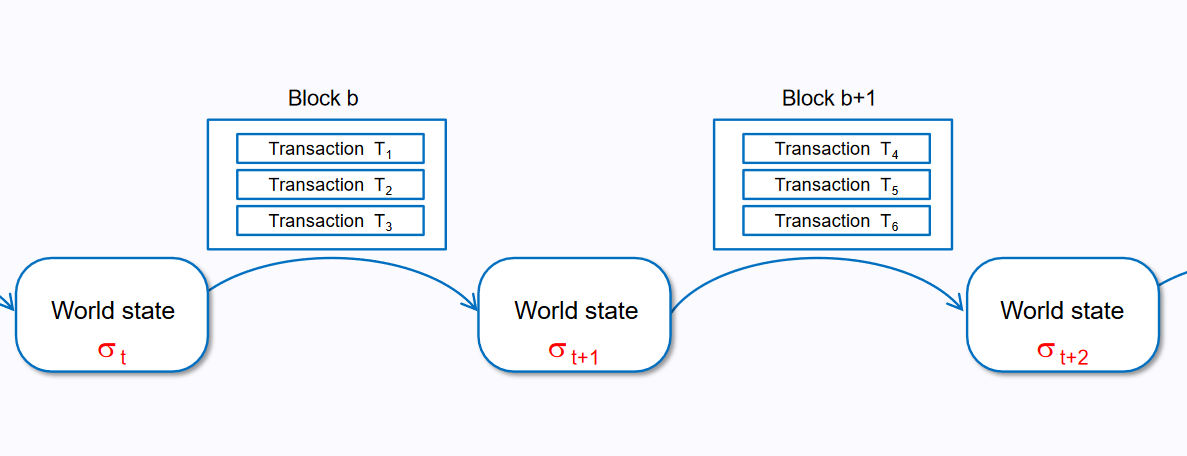
\includegraphics[width=1.0\textwidth]{blockchain_transitions}
    \caption{Ethereum can be seen as a chain of states~\cite{visual}}
    \label{fig:worldstate_update}
\end{figure}

A valid state transition requires the appending of a new block to the existing list of blocks. Each block contains transactions and a reference~to the previous block, forming a chain. In Ethereum, the only way for a block to be validated and appended to the list is through a validation process called mining. Mining involves a group of computers, known as miners, expending their computational resources to find the solution to a puzzle. The first miner to find a solution to the puzzle is rewarded with Ether\footnote{The Ethereum network's native currency} and is able to validate their block proposal. This is a process known as \textit{Proof of Work} (PoW) \cite{pow}. 

Due to a large number of miners competing to solve the PoW puzzle, sometimes a miner might solve the PoW at the same time with another miner, but for different block contents. This results in a \textit{fork} of the blockchain. Nodes will accept the first valid block that they receive\footnote{This depends on block propagation time based on bandwith, block-size, connectivity etc.}. Each blockchain protocol has a way to resolve forks and determine which chain is the valid chain. In Ethereum the longest chain is based on total difficulty\footnote{Difficulty is a measure of how much computational effort needs to be performed by a miner to solve a PoW puzzle. Total Difficulty is the sum of the difficulties of all blocks until the examined block.} which can be found in the \textit{blockheader}. Ethereum is advertised to be using a modification of the GHOST Protocol \cite{GHOST} as its chain selection mechanism which uses \textit{uncle blocks}\footnote{In Bitcoin a block with a valid PoW that arrived to a node after another valid block at the same height is called an orphan because it gets discarded by Bitcoin's algorithm. In Ethereum these blocks do not get discarded; instead they are added to the chain as \textit{uncle blocks} and receive a reduced block reward}. This is contradictory since Ethereum's uncle blocks do not count towards difficulty and as a result, Ethereum does not actually use an adaptation of the GHOST protocol \cite{Gervais:2016:SPP:2976749.2978341}; the uncle reward is just used to reduce miner centralization.

\begin{figure}[H]
    \centering
    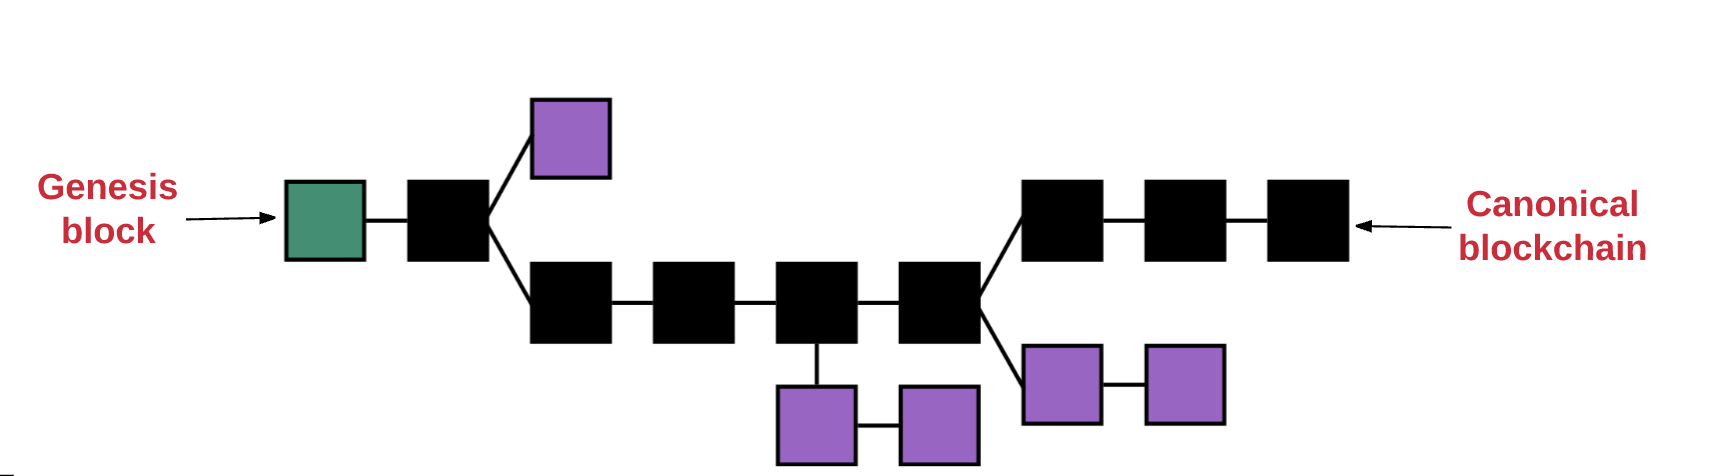
\includegraphics[width=1.0\textwidth]{fork}
    \caption{The Ethereum protocol chooses the longest chain~\cite{preethi}}
    \label{fig:forking}
\end{figure}

\section{Inside the Ethereum Virtual Machine}
\label{ch:basics:insideevm}
% https://hudsonjameson.com/2017-06-27-accounts-transactions-gas-ethereum/
The \textit{Ethereum Virtual Machine} (EVM) is the runtime environment for Ethereum. It is a Turing Complete State machine, allowing arbitrarily complex computations to be executed on it. Ethereum nodes validate blocks and also run the EVM, which means executing the code that is triggered by the transactions. In this section we go over the internals of the EVM\@. 

\subsection{Accounts}

\subsubsection*{World State}
Ethereum's world state is a mapping between addresses of accounts and their states. Full nodes download the blockchain, execute and verify the full result of every transaction since the genesis block. Users should run a full node if they need to execute every transaction in the blockchain or if they need to swiftly query historical data. 

\begin{figure}[H]
    \centering
    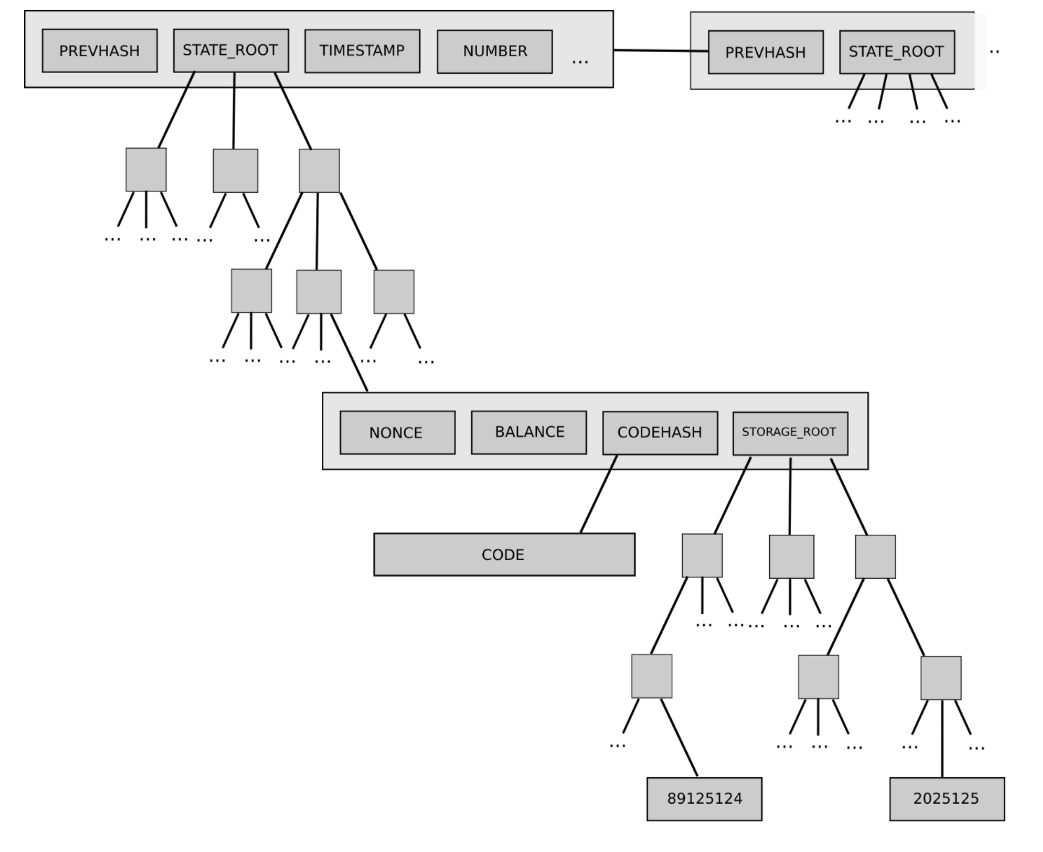
\includegraphics[width=1.0\textwidth]{world_state}
    \caption{The Ethereum world state~\cite{vitalik}}
    \label{fig:worldstate}
\end{figure}

A different kind of node called \textit{light node} exists for cases where there is no need to store all the information. Instead, light nodes use efficient data structures called \textit{Merkle Trees} which allow them to verify the validity of the data of a tree without storing the entire tree. A \textit{Merkle Tree} is a binary tree where each parent node is the hash of its two child nodes\footnote{Exception: Each leaf node represents the hash of a transaction in a block}. 

\begin{figure}[H]
    \centering
    \includegraphics[width=1.0\textwidth]{Merkle_tree}
    \caption{Node calculation in a Merkle Tree~\cite{smartproperty}}
    \label{fig:Merkletree}
\end{figure}


That way, instead of storing the whole tree of transactions, nodes can verify if a transaction was included in a block or not, just by checking if the `Merkle path' to the Merkle root is valid. This is efficient as there are only $O(lg_{2}(n))$ comparisons needed to check the validity of a transaction, as shown in Figure \ref{fig:Merkleproof}

\begin{figure}[H]
    \centering
    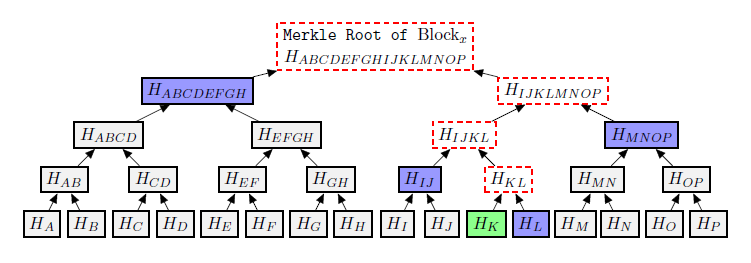
\includegraphics[width=1.0\textwidth]{merkle_proof}:
    \caption{Merkle path calculation~\cite{smartproperty}}
    \label{fig:Merkleproof}
\end{figure}


\subsubsection{Account State}
An ethereum account is a mapping between an address and an account state. There are two kinds of accounts, \textit{Externally Owned Accounts} (EOA) and \textit{Contract Accounts} (CA). EOAs are controlled by their Private Key and cannot contain EVM code. CAs contain EVM code and are controlled by the EVM code,

\begin{figure}[H]
    \centering
    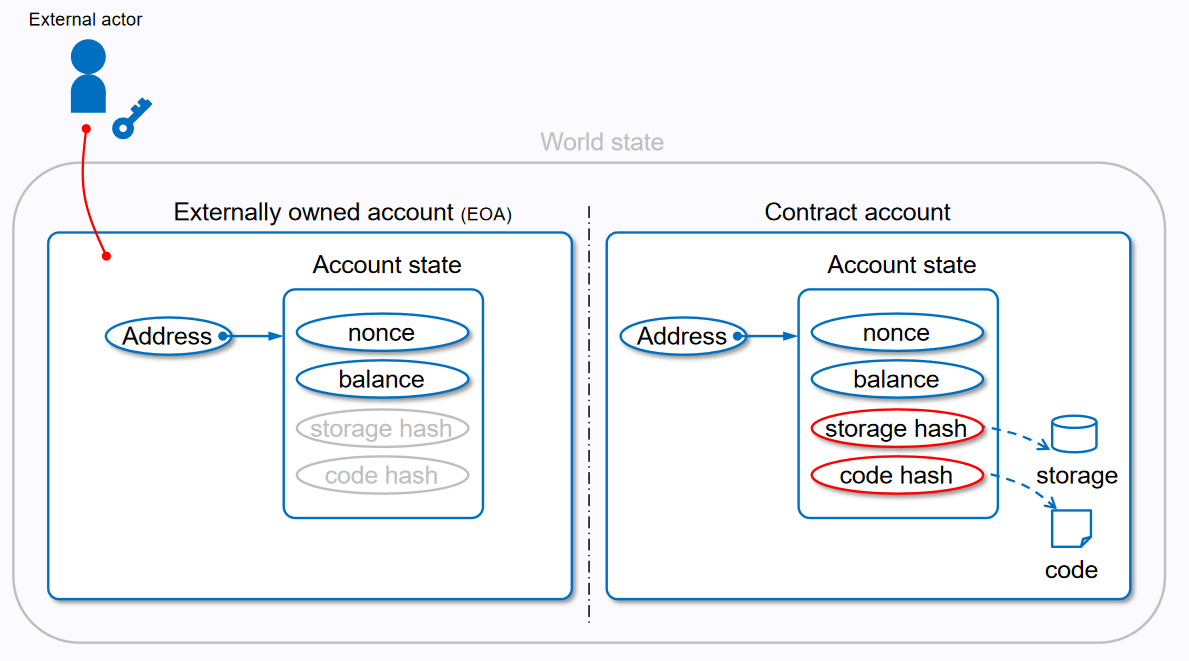
\includegraphics[width=1.0\textwidth]{accounts}
    \caption{Externally Owned Accounts and Contract Accounts in the Ethereum World state~\cite{visual}}
    \label{fig:accounts}
\end{figure}


An EOA is able to send a message to another EOA by signing a transaction with their private key. CAs can make transactions in response to transactions they receive from EOAs. 

\begin{figure}[H]
    \centering
    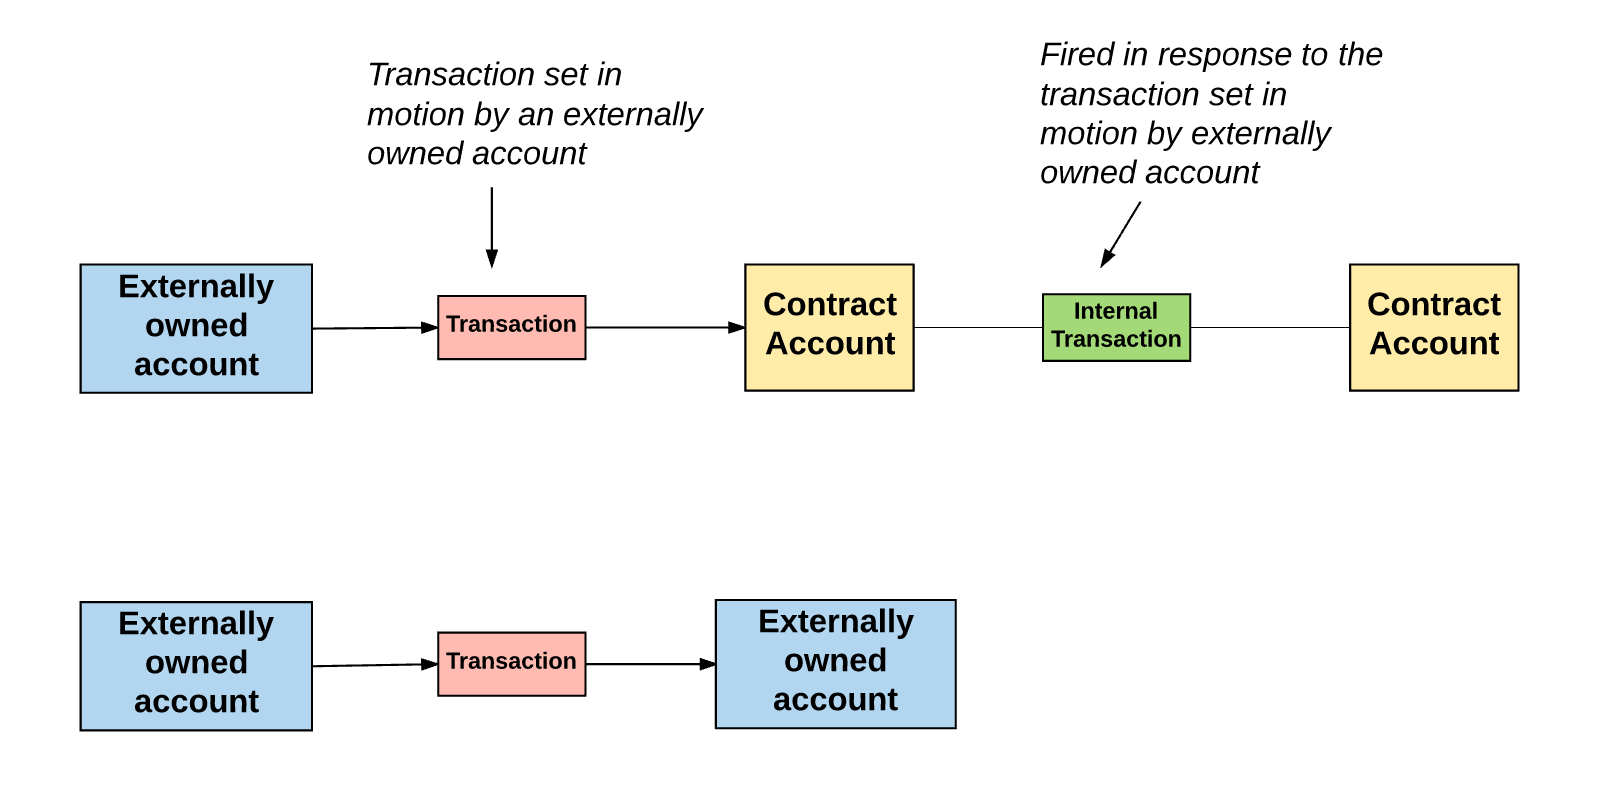
\includegraphics[width=1.0\textwidth]{result_tx}
    \caption{Transaction made by an EOA to an EOA or a contract~\cite{preethi}}
    \label{fig:tx_accounts}
\end{figure}

The public key of an EOA is derived from the private key through elliptic curve multiplication. The address of an EOA is calculated by calculating the KECCAK-256 hash of the public key and prefixing its last 20 bytes with `0x' \cite{ethereum}. The address of a CA is deterministically computed during contract creation from the sender EOA account's address and their transaction count\footnote{Full explanation: \url{https://ethereum.stackexchange.com/a/761}}.

We describe the contents of the Account State shown in Figure \ref{fig:accounts} as follows:
\begin{enumerate}
    \item \textbf{Nonce:} The number of transactions sent if it's an EOA, or the number of contracts created if it's a CA.
    \item \textbf{Balance:} The account's balance denominated in `wei'\footnote{1 ether $= 10^{18}$ wei }
    \item \textbf{Storage Hash:} The Merkle root of the account's storage contents. This is empty for EOAs
    \item \textbf{Code Hash:} The hash of the code of the account. For EOAs this field is the KECCAK-256 hash of the empty string (`') while for CAs it is the KECCAK-256 of the bytecode that exists at the CAs address.
\end{enumerate}

\subsection{Transactions} \label{transactions}
A transaction is a specially formatted data structure that gets signed by an EOA\footnote{With the EOAs private key} and gets broadcasted to an Ethereum node. Figure \ref{fig:transaction} shows the contents of a transaction as seen after querying an Ethereum node for its contents.

% In Bitcoin, the state is created through the Unspent Transaction Outputs set, which defines the amount of BTC  a user can spend. As Ethereum does not use UTXO but an account model, there needs to be a way to monitor the state. This is done through a data structure called Patricia State Trie \cite{Morrison:1968:PAR:321479.321481} which provides an efficient mapping of key and value pairs where the key is the address of the Ethereum account and the value is the Recursive Length Prefix encoding \cite{rlp} of the account's data. % TODO: Explain further or not? https://medium.com/cybermiles/diving-into-ethereums-world-state-c893102030ed %Whenever a transaction gets successfully mined, the world state gets updated accordingly.

Specifically:
\begin{enumerate}
    \item \textbf{blockHash:} The hash of the block that included the transaction.
    \item \textbf{blockNumber:} The number of the block that included the transaction.
    \item \textbf{from:} The transaction's sender\footnote{This field does not actually exist in a transaction however it is recovered from the v,r,s values of the signing algorithm (through \textit{ecrecover})}.
    \item \textbf{gas:} The maximum amount of gas units (hereafter referred to as \textit{gas}) that the sender will supply for the execution of the transaction (see \ref{gas}).
    \item \textbf{gasLimit:} The amount of Wei paid by the sender per unit of gas.
    \item \textbf{hash:} The transaction hash.
    \item \textbf{input:} Contains the data which is given as input to a smart contract in order to execute a function. Can also be used to embed a message in the transaction. Contains the value `0x0' in the case of simple transactions of ether.
    \item \textbf{nonce:} The number of transactions sent by the sender. It is used as a replay protection mechanism.
    \item \textbf{v, r, s:} Outputs of the ECDSA signature.
\end{enumerate}

\subsection{Blocks} \label{block}
A block contains the block header and a list of transaction hashes for all of the included transactions in that block. Figure \ref{fig:block} shows the contents of a transaction as seen after querying an Ethereum node for its contents.

Specifically:
\begin{enumerate}
    \item \textbf{difficulty:} The difficulty of the block.
    \item \textbf{extraData:} Extra data relevant to the block. Miners use it to claim credit for mining a block. In Bitcoin fields with extra data are used to let miners vote on a debate.
    \item \textbf{gasLimit:} The current maximum gas expenditure per block.
    \item \textbf{gasUsed:} The cumulative amount of gas used by all transactions included in the block.
    \item \textbf{hash:} The block's hash.
    \item \textbf{logsBlom:} A bloom filter which is used for getting further information from the transactions included in the block.
    \item \textbf{miner:} The address of the entity who mined the block.
    \item \textbf{mixHash:} A hash used for proving that the block has enough PoW on it.
    \item \textbf{nonce:} A number which when combined with the mixHash proves the validity of the block.
    \item \textbf{number:} The block's number.
    \item \textbf{parentHash:} The hash of the previous block's headers.
    \item \textbf{receiptsRoot:} The hash of the root node of the Merkle Tree containing the receipts of all transactions in the block .
    \item \textbf{sha3Uncles:} Hash of the uncles included in the block.
    \item \textbf{size:} Block size.
    \item \textbf{stateRoot:} The hash of the root node of the Merkle Tree containing the state (useful for light nodes).
    \item \textbf{totalDifficulty:} The cumulative difficulty of all mined blocks until the current block.
    \item \textbf{transactionsRoot:} The hash of the root node of the Merkle Tree containing all transactions in the block. 
\end{enumerate}

\subsection{Gas} \label{gas}
Since all nodes redundantly process all transactions and contract executions, an attacker would be able to maliciously flood the network with computationally intense transactions and cause nodes to perform costly operations for extended periods of time. Ethereum uses gas to introduce a cost on performing computations. Gas manifests itself as the fees to be paid by the sender for a transaction to complete successfully.

Every computational step on Ethereum costs gas. The simplest transaction which involves transferring Ether from one account to another costs 21000 gas. Calling functions of a contract involves additional operations where the costs can be estimated through the costs described in~\cite{gas, ethereum}. 

When referring to blocks, the \textit{gasLimit} is the maximum gas that can be included in a block. Since each transaction consumes a certain amount of gas, the cumulative gas used by all transactions in a block needs to be less than \textit{gasLimit}. There is a similarity between the block gasLimit and the block size in Bitcoin in that they are both used to limit the amount of transactions that can be included in a block. The difference in Ethereum is that miners can `vote' on the block gasLimit.

Every unit of gas costs a certain amount of \textit{gasPrice} which is set by the sender of the transaction. The cost of a transaction in wei is calculated from the formula
\begin{equation}\label{}
    totalTransactionCost = gasPrice * gasUsed
\end{equation}
where $gasUsed$ is the amount of gas consumed by the transaction.

Miners are considered to be rational players who are looking to maximize their profit. As a result, they are expected to include transactions with transaction costs before transactions with low transaction costs. This effectively creates a `fee market'  where users are willing to pay more by increasing the \textit{gasPrice} to have their transactions confirmed faster. In the times of network congestion such as popular Initial Coin Offerings\footnote{Crowdfunding for cryptocurrency projects which allow investors to buy tokens in a platform}\cite{batico} or mass-driven games such as CryptoKitties\footnote{\url{https://cryptokitties.co}}\cite{cryptokitties} transactions become very expensive and can take long times to confirm.

\subsubsection{Successful Transaction}
In the case of a successful transaction, the consumed gas from \textit{gasLimit} (\textit{gasUsed}) goes to miners, while the rest of the gas gets refunded to the sender. After the completion, the world state gets updated.

\begin{figure}[H]
    \centering
    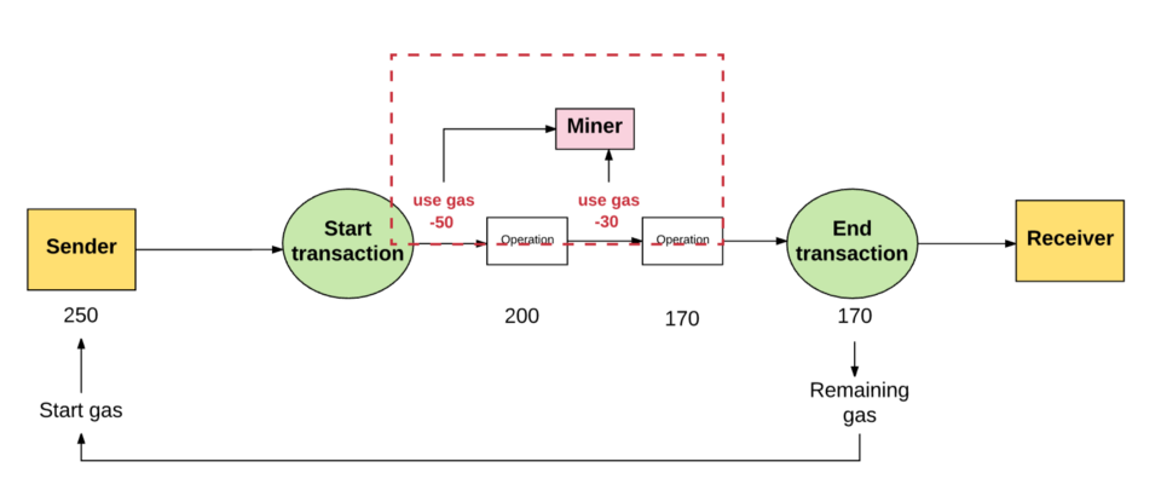
\includegraphics[width=1.0\textwidth]{successful_tx}
    \caption{Successful transaction~\cite{preethi}}
    \label{fig:successful_tx}
\end{figure}

\subsubsection{Failed Transaction}
A transaction can fail for reasons such as not being given enough gas for its computations, or some exception occurring during its execution. In this case, any gas consumed goes to the miners and any state changes that would happen are reverted. This is similar to the SQL transaction commit-rollback pattern.

\begin{figure}[H]
    \centering
    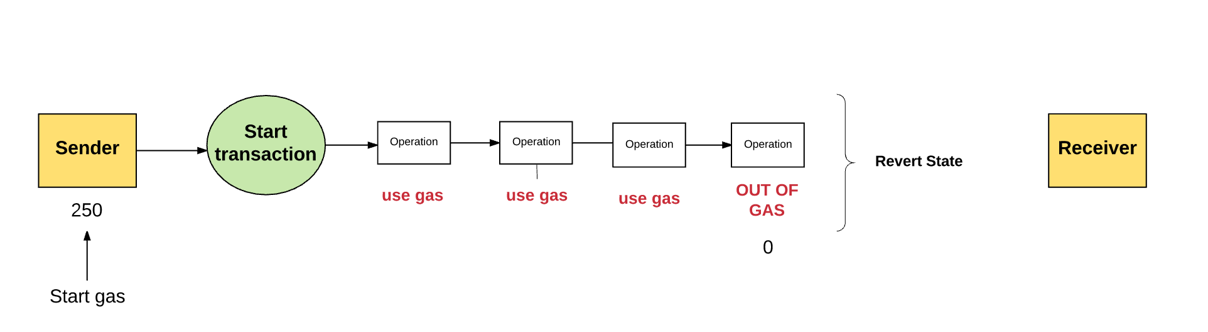
\includegraphics[width=1.0\textwidth]{nogas_tx}
    \caption{Failed transaction that ran out of gas, from \cite{preethi}}
    \label{fig:nogas_tx}
\end{figure}

\subsection{Mining}
The set of rules which allow an actor to add a valid block to the blockchain is called a \textit{consensus algorithm}. In order to have consensus in distributed systems, all participating nodes must have the same version (often called history) of the system. If there were no rules for block creation, a malicious node would be able to consistently censor transactions or double-spend \cite{doublespend}. In order to avoid that, consensus algorithms elect a network participant to decide on the contents of the next block. 

Ethereum uses a consensus algorithm called ethash\cite{ethash} which is a memory-hard\footnote{Requires a large amount of memory to execute it. This means that creating ASICs for ethash is harder, although not impossible \cite{asicfork}} consensus algorithm which requires a valid PoW in order to append a block to the Ethereum blockchain. PoW involves finding an input called \textit{nonce} to the algorithm so that the output number is less than a certain threshold\footnote{The threshold is also called difficulty and adjusts dynamically so that a valid PoW is found approximately every 12.5 seconds}. PoW algorithms are designed so that the best strategy to find a valid nonce is by enumerating through all the possible options. Finding a valid PoW is a problem that requires a lot of computational power, however verifying a solution is a trivial process, given the nonce. In return, miners are rewarded with the \textit{block reward} and with all the fees from the block's transactions.

This process is called `mining'. In the future, Ethereum is planning to transition to another \textit{consensus algorithm} called Proof of Stake (PoS), which deprecates the concept of `mining' and replaces it with `staking'. PoS is considered to be a catalyst for achieving scalability in blockchains and is briefly discussed in Chapter \ref{ch:scalability}.

%%%%%%%%%%%%%%%%%%%%%%%%%%%%%%%%%%%%%%%%%

\section{Programming in Ethereum}
At a low level, the EVM has its own Turing Complete language called the EVM bytecode. Programmers write in higher-level languages and compile the code from them to EVM bytecode which gets executed by the EVM\@.

\subsection{Programming Languages}
Languages that compile to EVM code are Solidity, Serpent, LLL or Vyper. Active research is being done towards more safe and secure smart contract languages~\cite{bamboo, flint}. Solidity is the most popular language in the ecosystem and although often comparable to Javascript, we argue that Solidity Smart Contracts remind more of C++ or Java, due to their object oriented design. The Solidity Compiler is called \texttt{solc}. In order to deploy a smart contract, its EVM Bytecode and its Application Binary Interface (ABI) are needed, which can be obtained from the compiler.

\begin{figure}[ht]
    \centering
    \lstinputlisting[language=Solidity]{contracts/example1.sol}
    \caption{Basic Solidity Smart Contract}
    \label{fig:smart_contract}
\end{figure}

\subsection{Tooling}
The following section describes tools and software that are often used by Ethereum users and developers to interact with the network.

\subsubsection{Client Implementations and Testnets}
Ethereum's official implementations are Geth (golang) and cpp-ethereum (C++). Third party implementations such as Parity (Rust), Pyethereum (Python) and EthereumJ (Java) also exist. The most used kind of node implementations are Geth (compatible with Rinkeby testnet) and Parity (compatible with Kovan testnet). 

Smart contracts are immutable once deployed which means that their deployed bytecode (and thus their functionality) cannot change. As a result, if a flaw is found on a deployed contract, the only way to fix it is by deploying a new contract. In addition, the deployment costs can be expensive, so development and iterative testing can be costly. For that, public test networks (testnets) exist which allow for testing free of charge. Kovan and Rinkeby are functioning with the Proof of Authority \cite{poa} consensus algorithm, while Ropsten is running Ethash \cite{ethash} with less difficulty.

We provide a listing of the currently public test networks:
\begin{enumerate}
    \item Kovan: Proof of Authority consensus supported by Parity nodes only
    \item Rinkeby: Proof of Authority consensus supported by Geth nodes only
    \item Ropsten: Proof of Work consensus, supported by all node implementations, provides best simulation to the main network 
    % https://ethereum.stackexchange.com/questions/27048/comparison-of-the-different-testnets
\end{enumerate}
% https://ethereum.stackexchange.com/questions/27048/comparison-of-the-different-testnets

In addition, before deploying to a testnet, developers are encouraged to run their own local testnets. Geth and Parity allow for setting up private testnets. Third-party tools also exist that allow for setting up a blockchain with instant confirmation times and prefunded accounts, such as ganache\footnote{\url{http://truffleframework.com/ganache}}(User Interface at \ref{fig:ganache},  formerly known as testrpc).


\subsubsection{Web3}
Web3 is the library used for interacting with an Ethereum node. The most feature-rich implementation is Web3.js\footnote{\url{https://github.com/ethereum/web3.js}} which is also used for building web interfaces for Ethereum Decentralized Applications (DApps). Implementations for other programming languages are being worked on such as Web3.py\footnote{\url{https://github.com/ethereum/web3.py}}. We illustrate an example of connecting and fetching the latest block from Ropsten and Mainnet using Web3.js in \ref{fig:web3js} and Web3.py in \ref{fig:web3py}. The full specifications of each library's API can be found in their respective documentation\footnote{\url{https://github.com/ethereum/wiki/wiki/JavaScript-API}}\footnote{\url{https://web3py.readthedocs.io/en/stable/}}


\subsubsection{Truffle Framework}
The Truffle Framework is a development framework for smart contract development written in NodeJS. It is currently the industry standard for developers. It allows for automating the smart contract deployment pipeline through \textit{migration} scripts and scripting test suites for scenarios using the Mocha Testing suite. Finally, it includes a debugger for stepping through transaction execution and can internally launch a ganache testnet.

\section{Related Work}
Techniques which illustrate more efficient smart contracts by storing less data on a blockchain are described in~\cite{stateless}. With this method, it is possible to store the data in the input of a transaction, removing the need of smart contract. The data can then be processed in an application by watching for transactions that get sent to the contract's address and decoding their inputs. 

% Network Level Scalability
On network level scalability there are various approaches such as executing transactions `off-chain'\footnote{An exchange of cryptographically signed messages that does not happen on a blockchain.} and use a blockchain only for the final settling of a series of transactions by utilizing a technique called payment channels~\cite{lightning, raiden, funfair, counterfactual}. Other approaches exist which involve creating `sidechains' which can be utilized to perform trustless computation on another blockchain, that is pegged to the security of the root chain~\cite{sidechains, loom, cosmos, plasmacash, plasma}. Finally, another approach to achieving scalability is via permissioned blockchains which trade decentralization and transparency for efficiency~\cite{hyperledger, Vukolic:2017:RPB:3055518.3055526}.

% Contract Level Scalability
Cheng et al make it clear that compiler optimizations in smart contracts still need improvements in order to avoid unnecessary expenses \cite{DBLP:journals/corr/ChenLLZ17}. They identify 7 gas-costly patterns and develop a tool called GASPER that is able to identify 3 of these patterns from the bytecode of already deployed smart contracts. The evaluation of the frequency of these patterns show that over 70\% of the deployed smart contracts on Ethereum until Nov. 5th. 2016 suffer from these 3 patterns. Although experienced software engineers can avoid these bad practices, the compiler should be able to detect and optimize parts of the code which are unreachable, and not perform redundant operations.

% Security tools
Extensive analyses have been performed on the security of blockchains as networks and specifically on the security of Ethereum smart contracts~\cite{Gervais:2016:SPP:2976749.2978341, Atzei:2017:SAE:3080353.3080363}. While the Ethereum network as a Proof of Work blockchain has not been successfully attacked since its inception, Smart contracts have proven to be insufficiently secure for the amounts of funds that they hold, with large amounts of funds being stolen in multiple occurences \cite{parityhack, paritypostmortem, hackingdistibuteddao}. As a result, tools that are able to analyze both source code and compiled bytecode for vulnerabilities have been developed~\cite{Luu:2016:MSC:2976749.2978309, mythril, echidna, smartcheck, securify, zeus}. A recent study identifies `greedy', `prodigal' and `suicidal' smart contracts that can freeze or cause loss of funds, however there has been criticism on the validity of the authors' findings \cite{greedyprodigal, criticismgreedyprodigal}.

% Use case
Utilizing blockchain for Internet of Things is explored in \cite{iot, integrationiot}, while a model for billing and accounting with smart contracts is proposed in~\cite{billaccount}. In all cases, it is acknowledged that existing blockchain infrastructure cannot support the amount of transaction load that is needed by the IoT ecosystem. Energy market use-cases are being piloted by introducing peer to peer energy market trading, while utilizing hardware agents to facilitate the energy management~\cite{gridplus, powerledger}. Finally, microgrid blockchain prototypes are being tested such as \cite{brooklyn, DBLP:journals/ife/MengelkampNBDW18}.
\chapter{Blockchain Scalability}\label{ch:scalability}

\section{Bottlenecks in Scalability}
A blockchain's ability to scale is often measured by the amount of transactions it can verify per second. A block gets appended to the Ethereum blockchain every 12.5 seconds on average, and can contain only a finite amount of transactions. As a result, transaction throughput is bound by the frequency of new blocks and by the number of transactions in them.

We argue that there are two levels of scalability, scalability on contract and on network level. Better contract design can result in transactions which require less gas to execute, and thus allow for more transactions to fit in a block while also making it cheaper for the end user.With Ethereum's current blockGasLimit at 8003916, if all transactions in Ethereum were simple financial transactions\footnote{Not calls to smart contracts. Transactions without any extra data cost 21000 gas}, each block would be able to verify ~381 transactions, or 25 transactions per second (tps), which is still not comparable to traditional payment operators. 

\section{Network Level Scalability}
Scale should not be confused with scalability. While scale describes the size of a system and the amount of data being processed, scalability describes how the cost of running the system changes as scale increases. Existing blockchains scale poorly due to the costs associated with them increase faster than the rate at which data can be processed. 

First of all, transactions per second as a metric is inaccurate. Solving scalability does not imply just increasing the transaction throughput. It is a constraint-satisfaction-problem; the goal is to maximize throughput while maintaining the network's decentralization and security. 

\begin{figure}[H]
\begin{quote}
    \textbf{This sounds like there’s some kind of scalability trilemma at play. What is this trilemma and can we break through it?}

    The trilemma claims that blockchain systems can only at most have two of the following three properties:

    \begin{itemize}
        \item Decentralization (defined as the system being able to run in a scenario where each participant only has access to $O(c)$ resources, ie. a regular laptop or small VPS)
        \item Scalability (defined as being able to process $O(n) > O(c)$ transactions)
        \item Security (defined as being secure against attackers with up to $O(n)$ resources)
    \end{itemize}
\end{quote}
\label{fig:trilemma}
\caption{The Scalability Trilemma, from Ethereum's Sharding documentation \cite{sharding}}
\end{figure}

An example that trades decentralization for more transactions is increasing the block size so that more transactions can fit inside a block and thus increase throughput. Increasing the size of each block, implies more disk space for storing the blockchain, better bandwith for propagating the blocks and more processing power on a node to verify any performed computations. This eventually requires computers with datacenter-level network connections and processing power which are not accessible to the average consumer, thus damaging decentralization which is the core value proposition of blockchain. % The blockGasLimit can be voted on by miners\footnote{\url{https://www.etherchain.org/tools/gasLimitVoting}}. % In addition to the reasons stated above, increasing the gas limit also potentially damages the security of the network due to increased uncle rates, Ethereum's analog to Bitcoin's orphan blocks \footnote{\url{https://blockchain.info/orphaned-blocks}}. Longer propagation time implies that a miner will spend more time searching for a solution until they receive a valid block, and thus has more chances of finding a valid block in that time. As a result, 

As described in \cite{scaling-trustless-models}, Proof of Work is a consensus algorithm optimized for censorship-resistance while (in theory) maintain a low barrier to entry, as shown in Figure \ref{fig:scalability_triangle_pow}. In reality, due to economies of scale, PoW blockchains end up being centralized around small numbers of miners \cite{Gencer2018DecentralizationIB}. 

\begin{figure}[ht!]
    \centering
    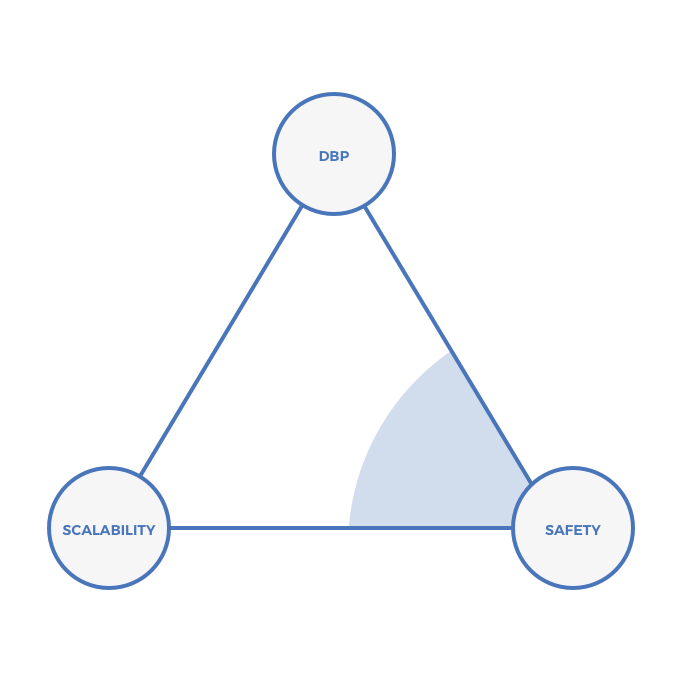
\includegraphics[width=0.5\textwidth]{scalability_triangle_pow}
    \caption{Bitcoin and Ethereum's PoW networks have slow probabilistic time to finality and do not scale well. Mining capacity has high concentration in a small amount of entities, from \cite{scaling-trustless-models}}
    \label{fig:scalability_triangle_pow}
\end{figure}

We proceed to discuss some network level solutions that can improve Ethereum's scalability.

\subsubsection*{Proof of Stake}
Proof of Stake (PoS) is an alternative consensus algorithm where in the place of miners, there are validators who instead of expending computational resources to `mine' a valid block, they stake\footnote{Lock up for an amount of time} their ether and the probability for them to be elected to validate the next block is proportional to their stake. Designing a secure PoS protocol is still under heavy research. The Ethereum Foundation is working on `Casper the Friendly Finality Gadget'~\cite{casperffg} which is a hybrid PoW/PoS consensus algorithm that provides block finality\footnote{A block that is finalized cannot be reverted. This is different to traditional PoW which achieves \textit{probabilistic finality}; a block is considered harder to revert the older it is.} which combined with the `correct-by-construction Casper the Friendly GHOST'\footnote{Uses the GHOST protocol to choose a chain in the case of a fork.} \cite{caspertfg} will enable a full transition to Proof of Stake. 

\subsubsection*{Sidechains}
A sidechain~\cite{sidechains} is a blockchain defined by a custom `rule-set' and can be used to offload computations from another chain. Individual sidechains can follow different sets of rules from the mainchain, which means they can optimize for applications that require high speeds or heavy computation, while still relying on the mainchain for issues requiring the highest levels of security. Ethereum's sidechain solution is called `Plasma' \cite{plasma} and involves creating \textit{Plasma chains} that run their own consensus algorithm and communicate with the mainchain via a two-way peg as described in \cite{sidechains}. \textit{Plasma chains} can have more adjustable parameters such as be less decentralized, however the protocol does not allow for the Plasma Chain operator to abuse their power. A more recent Plasma construct is called `Plasma-Cash' \cite{plasmacash} and describes a more efficient way of executing fraud proofs, in the case of a malicious actor in a \textit{Plasma chain}.

\subsubsection*{Sharding}
Due to the architecture of the EVM all transactions are executed sequentially on all nodes. Sharding~\cite{sharding} refers to splitting the process across nodes, so that each full node is responsible only for a shard\footnote{A shard is a part of the blockchain's state} and acts as a light client to the other shards. Sharding is the most complex scaling solution and is still at research stages. It also requires a stable Proof of Stake consensus algorithm to function properly.

\subsubsection*{State channels}
Contrary to the previous solutions which still record messages on a blockchain, state channels involves exchange of information `off-chain'. The primary use-case for state channels is micro-transactions between two or more parties. This technique involves exchanging signed messages through a secure communications channel and perform a transaction on the blockchain only when the process is done\footnote{Example: Instead of making 10 transactions worth 0.1 ether each, a transaction is made to open the channel, participants exchange off-chain messages transferring value, and settle or dispute the channel with one more transaction at the end.}.

\section{Contract Level Scalability}
In a recent study \cite{DBLP:journals/corr/ChenLLZ17}, after evaluating 4240 smart contracts, it is found that over 70\% of them cost more gas than they should due to the compiler failing to properly optimize the Solidity code during compilation. In this section we explore how gas gets computed in smart contracts and potential ways we can save on gas and transaction costs.

\subsection{Gas Costs}
An Ethereum transaction total gas costs are split in two: % https://ethereum.stackexchange.com/a/29560
\begin{enumerate}
    \item \textbf{Transaction Costs:} The cost of sending data to the blockchain. There are 4 items which make up the full transaction cost:
        \begin{enumerate}
            \item The base cost of a transaction (21000 gas). % hereafter gas units will be referred to as gas
            \item The cost of deploying a contract (32000 gas).
            \item The cost for every zero byte of data in a transaction input (4 gas per zero byte).
            \item The cost of every non-zero byte of data in a transaction input (68 gas per non-zero byte).
        \end{enumerate}
    \item \textbf{Execution Costs:} The cost of computational operations which are executed as a result of the the transaction, as described in detail in \cite{ethereum, gas}.
\end{enumerate} 

Gas costs get translated to transaction fees. As a result, a contract should be designed to minimize its operational gas costs in order to minimize its transaction fees. Transactions that cost less gas allow more room for other transactions to be included in a block which can improve scalability. % In addition, as gas is a unit for computational costs, less gas consumed results in less burden on the nodes validating the smart contracts which can lead to better scalability.

\begin{table}[H]
	\centering
	\vspace*{-1ex}
	\scriptsize
	\caption{Gas cost of different operations, a complete list can be found in Ethereum's yellow paper~\cite{gas}, from \cite{DBLP:journals/corr/ChenLLZ17}}
	\vspace{-1ex}
	\label{table:opcode_table}
	\begin{tabular}{|c|c|c|}
		\hline
		\textbf{Operation}        & \textbf{Gas} & \textbf{Description} \\ \hline
		\textsc{ADD/SUB}          & 3 & \multirow{3}{*}{Arithmetic operation} \\ \cline{1-2}
		\textsc{MUL/DIV}          & 5 & \\ \cline{1-2}
		\textsc{ADDMOD/MULMOD}    & 8 & \\ \hline
		\textsc{AND/OR/XOR}       & 3 & Bitwise logic operation \\ \hline
		\textsc{LT/GT/SLT/SGT/EQ} & 3 & Comparison operation \\ \hline
		\textsc{POP}              & 2 & \multirow{2}{*}{Stack operation} \\ \cline{1-2}
		\textsc{PUSH/DUP/SWAP}    & 3 & \\ \hline
		\textsc{MLOAD/MSTORE}     & 3 & Memory operation \\ \hline
		\textsc{JUMP}             & 8 & Unconditional jump \\ \hline
		\textsc{JUMPI}            & 10 & Conditional jump \\ \hline
		\textsc{SLOAD}            & 200 & \multirow{2}{*}{Storage operation} \\ \cline{1-2}
		\textsc{SSTORE}           & 5,000/20,000 & \\ \hline
		\textsc{BALANCE}          & 400 & Get balance of an account \\ \hline
		\textsc{CREATE}           & 32,000 & Create a new account using CREATE \\ \hline
		\textsc{CALL}             & 25,000 & Create a new account using CALL \\  \hline
	\end{tabular}
	\vspace{-2ex}
\end{table}

% bytecontracts includes constructor and general initialisation contracts which is not needed anymore at runtime. The contracts that is sent during deployment (bytecontracts), even excluding the constructor arguments, is - in general - different from the contracts that is stored at that address (the runtimeBytecontracts).

As seen in Table \ref{table:opcode_table}, the most expensive operations involve CREATE\footnote{Used to create a new contract.} and SSTORE operations. The focus of this section will be to explore ways to decrease gas costs on Smart Contracts, either through better practices or by handcrafting optimizations for specific use cases.

It should be noted, that non-standard methods have been proposed for reducing fees incurred by gas costs. A recent construction \cite{gastoken} describes a method of buying gas at low cost periods and saving it in order to spend it when gas prices are higher\footnote{When the network is congested}. The economic implications of gas arbitrage are outside the scope of this Master Thesis. 

General rules that should be followed for saving gas costs:
\begin{enumerate}
    \item Enable compiler optimizations (although can lead to unexpected scenarios~\cite{compiler}).
    \item Reuse code through libraries~\cite{library}.
    \item Setting a variable back to zero refunds 15000 gas through SSTORE, so if a variable is going to be unused it is considered good practice to call \texttt{delete} on it. 
    \item When iterating through an array, if the break condition involves the array's length set it as a stack variable the loop. This way, it doesn't get loaded during each loop and allows for saving 200 gas per iteration \cite{DBLP:journals/corr/ChenLLZ17}.
    \item Use \texttt{bytes32} instead of \texttt{string} for strings that are of known size. \texttt{bytes32} always fit in an EVM word, while \texttt{string} types can be arbitrarily long and thus require more gas for saving their length.
    \item Do not store large amounts of data on a blockchain. It is more efficient to store a hash which can be either proof of the existence of the data at a point in time, or it can be a hash pointing to the full data\footnote{This pattern has been used in combination with IPFS, \url{https://ipfs.io}}
\end{enumerate}

As described in \cite{DBLP:journals/corr/ChenLLZ17} there is a lot of room for further compiler optimizations. Future Solidity compiler versions are addressing some already\footnote{\url{https://github.com/ethereum/solidity/issues/3760}}\footnote{\url{https://github.com/ethereum/solidity/issues/3716}}\footnote{\url{https://github.com/ethereum/solidity/issues/3691}}

The EVM operates on 32 byte (256 bit) words. The compiler is able to `tightly pack' data together, which means that 2 128 bit storage variables can be efficiently stored with 1 SSTORE command. The \textit{optimize} flag of the Solidity compiler needs to be activated to access this feature when programming in Solidity. Refer to \ref{fig:struct_optimization} for an example of the optimizer's functionality.

\subsection{Gas Savings Case Study}

We proceed to compare the gas efficiency of 3 methods for storing data in a smart contract based on a gaming use-case. The contract-design requirements are: 
\begin{itemize}
    \item A user must be able to register.
    \item A user must be able to create a character with certain traits as function arguments.
    \item A user must be able to retrieve the traits of a character.
\end{itemize}

\begin{table}[H]
	\centering
	\vspace*{-1ex}
	\scriptsize
	\vspace{-1ex}
	\begin{tabular}{|c|c|c|}
        \hline
        \textbf{Name} & \textbf{Type}  & \textbf{Comment}\\ \hline 
        playerID      & uint16         & Game supports up to 65535 players\\
        creationTime  & uint32         & Game supports timestamps up to 2**32 = 02/07/2106 @ 6:28am (UTC) \\
        class         & uint4          & Game supports up to 16 classes \\
        race          & uint4          & Game supports up to 16 classes \\
        strength      & uint16         & Stats can be up to 65535\\
        agility       & uint16         & Stats can be up to 65535 \\
        wisdom        & uint16         & Stats can be up to 65535 \\
        metadata      & bytes18        & Utilize the rest of the word for metadata \\
        \hline
    \end{tabular}
	\caption{Required variables and size. Sizes add up to 248 bits which can be efficiently stored in a 256 bit word.}
    \label{table:characteristics}
\end{table}


The choice of variables is made to represent what the traits of a character would be in a game built on a smart contract. The size of the variables is selected so that all the information required to describe a \texttt{Character} can fit in a 256 bit word. The interface that satisfies the requirements is shown in~\ref{fig:game_interface}.

For each of the following implementations we will examine the deployment gas costs, as well as the gas costs for calling each function:

\begin{enumerate}
    \item Packing of traits through structs relying on the optimizer.
    \item Manually pack traits in a \texttt{uint256} variable with masking and shifting.
    \item Manually pack traits in a \texttt{bytes32} variable (equivalent in length to \texttt{uint256}) with masking and shifting, utilizing Solidity Libraries, influenced by~\cite{virtualstruct}.
\end{enumerate}
We use \texttt{bytes32} in Method 3 because the bit operations done in Solidity when extracted in functions do not function as expected with \texttt{uint256} variables. The full contract implementations for each method can be found in Appendix \ref{apx:scalability}. A side-by-side comparison of each method is shown in \ref{ch:scalability:results}% In this section we describe the methods and in section \label{results} we go over the results and caveats of each method.

\subsubsection{Method 1: Packing of traits through structs relying on the optimizer} \label{method1}
We use Solidity's built-in \texttt{struct}\footnote{\url{http://solidity.readthedocs.io/en/v0.4.21/types.html}} keyword as means to group all traits of a \texttt{Character} as described in \ref{table:characteristics}. This allows for easy code readability since every variable of a \texttt{struct} can be accessed by its name as seen in \ref{fig:struct_optimization:c}, like the property of an object. 

In this case, assignment and retrieval of the variables is done in a very straightforward way. By utilizing Solidity's built-in structures and arrays, we can create an array of \texttt{Character} type structures and access their traits by their indexes, as done in \ref{fig:struct_optimization:c}

The gas costs per function call with this method are: 
\begin{table}[H]
	\centering
	\caption{Gas costs for deployment and for each function using Solidity's built-in structs}
	\vspace*{-1ex}
	\scriptsize
	\vspace{-1ex}
	\begin{tabular}{|c|c|c|c|}
		\hline
		\textbf{Optimizer Runs} & \textbf{Register} & \textbf{CreateCharacter} & \textbf{Deployment} \\ \hline
        0      &    70003 &          104205 &    903173.0 \\
        1      &    69943 &          104202 &    529979.0 \\
        100    &    69811 &          103402 &    561342.0 \\
        500    &    69604 &          103207 &    586867.0 \\
		500000 &    69598 &          103183 &    651665.0 \\
		\hline
    \end{tabular}
	\vspace{-2ex}
	\label{table:tightpacking}
\end{table}

\subsubsection{Method 2: Manually pack traits in a \texttt{uint256} variable with masking and shifting} \label{method2}
    
In \ref{method1} we rely on the optimizer to make storing a character's traits more efficient. It turns out\footnote{\url{https://github.com/figs999/Ethereum/blob/master/Solc.aComedyInOneAct}} that the optimizer is not able to remove all unnecessary operations and there is still room for improvement. In order to get better results, we create a local stack variable\footnote{The data is 248 bits long, so we create a \texttt{uint256} variable} which is large enough to store all the traits from \ref{table:characteristics}. Instead of creating a \texttt{struct}, we manually encode each trait in the said variable, essentially we act as the optimizer, which results in much less gas spent as both the contract's bytecode is smaller and the \texttt{text}{CreateCharacter} function is more efficient. We proceed to describe the encoding process.

By left shifting a trait's value by the sum of the size of all variables to its right and then performing a bitwise OR operation with the \texttt{uint256}, the trait gets encoded in the \texttt{uint256}, as shown in~\ref{fig:uint_encoding}. This is implemented in \ref{fig:uint_encoding_code}

\begin{figure}[H]
    \centering
    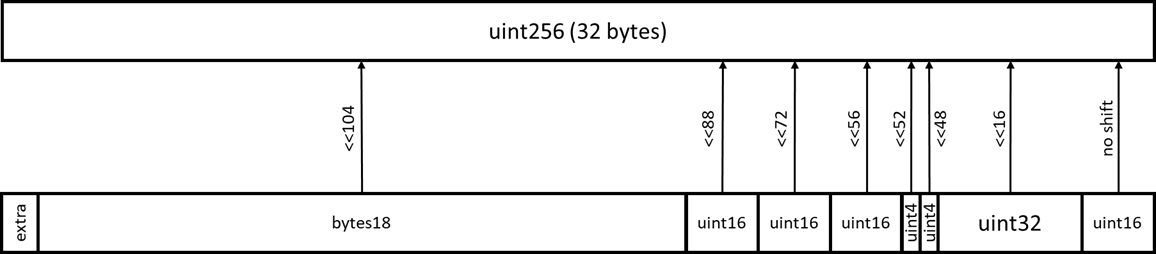
\includegraphics[width=\textwidth]{uint_encoding}
    \caption{Setting data requires shifting left $N$ times and performing bitwise OR with the target variable, where $N$ is the sum of the number of bits of all variables to the right of the target variable.}
    \label{fig:uint_encoding}
\end{figure}

By right shifting the \texttt{uint256} by the sum of the size of all variables to the right of a trait and then performing a bitwise AND operations with the trait's size retrieves the value of the trait. Figure \ref{fig:uint_decoding} illustrates retrieving the \texttt{creationTime} trait from the \texttt{uint256} by shifting right 16 times and performing bitwise AND with $2^32-1$ since \texttt{creationTime} is a 32 bit variable. This is implemented in \ref{fig:uint_decoding_code}.

\begin{figure}[H]
    \centering
    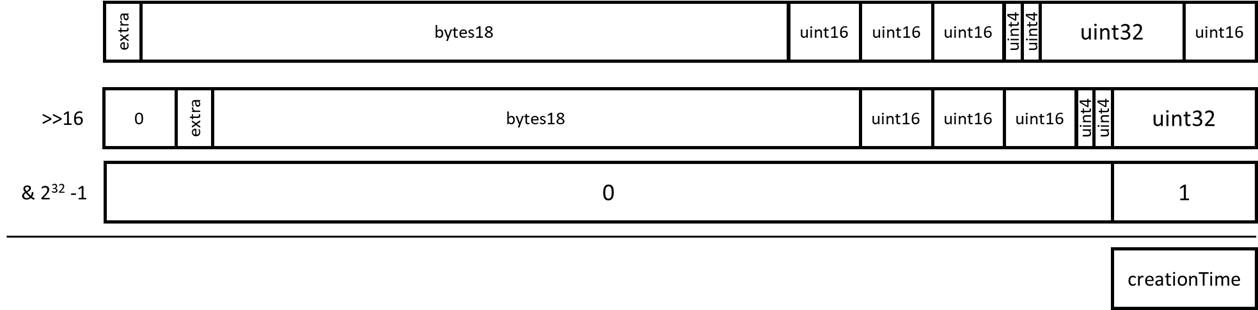
\includegraphics[width=\textwidth]{uint_decoding}
    \caption{Retrieving data requires shifting right $N$: times and performing bitwise AND with the target variable's size, where $N$ is the sum of the number of bits of all variables to the right of the target variable.}
    \label{fig:uint_decoding}
\end{figure}

The gas costs per function call with this method are: 
\begin{table}[H]
	\centering
	\caption{Gas costs for deployment and for each function using the masking method on a uint.}
	\vspace*{-1ex}
	\scriptsize
	\vspace{-1ex}
	\begin{tabular}{|c|c|c|c|}
		\hline
		\textbf{Optimizer Runs} & \textbf{Register} & \textbf{CreateCharacter} & \textbf{Deployment} \\ \hline
        0      &    70003 &           66620 &    551800.0 \\
        1      &    69943 &           66365 &    378022.0 \\
        100    &    69811 &           65924 &    402120.0 \\
        500    &    69604 &           65855 &    419559.0 \\
		500000 &    69598 &           65855 &    432409.0 \\
		\hline
	\end{tabular}
	\vspace{-2ex}
	\label{table:uint_masking_gas}
\end{table}

\subsubsection{Method 3: Manually pack traits in a bytes32 variable with masking and shifting, utilizing Solidity Libraries} \label{method3}

Code reusability and readability should always be given high priority. Although data packing is very efficient in~\ref{method2} compared to~\ref{method1}, the code is hardly readable and it is impossible to reuse parts of it. % It is possible to extract the logic into functions, however the overheads introduced by the additional operations make it inferior to the technique we describe in this section.
We utilize Solidity's \texttt{Library} built-in which allows us to define a set of methods which can be applied on a datatype using the \texttt{using X for Y} syntax\footnote{This is similar to calling functions on struct's in Golang}. A simple example is shown in \ref{fig:library}.

\begin{figure}[ht!]
    \centering
    \lstinputlisting[language=Solidity]{contracts/LibraryExample.sol}
    \caption{Example of using the \texttt{using X for Y} syntax to enhance operations done on datatypes.}
    \label{fig:library}
\end{figure}

The visibility of a Library's exported functions can be: 
\begin{enumerate}
    \item \textbf{Internal:}
        In this case, the compiled library's bytecode is inlined to the main contract's code. This results in larger bytecode during deployment, however each of the Library's functions are called via the \texttt{JUMP} opcode. In this case, only the base contract gets deployed.
    \item \textbf{Public:}
        In this case, the main contract's bytecode has placeholder slots. These slots get filled by the Library's address which is obtained after deploying the Library contract. After replacing the placeholder slots with the Library's address, any function call to the library is done via the \texttt{DELEGATECALL} opcode.
\end{enumerate}

% Should insert placeholder and inlined bytecode? 

Libraries with public functions are deployed as standalone contracts to be used by contracts made by other developers. They often include generic functionality such as math operations\footnote{A popular Solidity Library is SafeMath which contains error-checked math operations}. Depending on the complexity of the contracts, this can be more efficient compared to using \texttt{internal} functions. % When \textit{public} is used, the DELEGATECALL opcode is used\footnote{Relays the message to the library while allowing it to execute in the sender's state}. When \textit{internal} is used, a function call is interpreted as a jump and thus is more efficient than the DELEGATECALL. 

That way, instead of having to deploy a new contract, developers can use an already deployed one. Due to the usage of \texttt{DELEGATECALL}, there is a tradeoff between contract deployment costs and the extra costs incurred when making function calls. We use \texttt{internal} because it requires less gas and since this is a specialized use-case it is not expected to be used by third-parties.

The final version is split in two files, the library which includes the API for setting and retrieving the character's traits, and the main contract which uses the library's high-level functions. By utilizing the \texttt{using CharacterLib for bytes32} syntax we are able to store and retrieve a character's traits in a user-friendly manner.

The gas costs per function call with this method are: 
\begin{table}[H]
	\centering
	\vspace*{-1ex}
	\scriptsize
	\vspace{-1ex}
	\label{table:byte_masking_gas}
	\begin{tabular}{|c|c|c|c|}
		\hline
		\textbf{Optimizer Runs} & \textbf{Register} & \textbf{CreateCharacter} & \textbf{Deployment} \\ \hline
        0      &    70003 &           67581 &    754613.0 \\
        1      &    69943 &           67414 &    508014.0 \\
        100    &    69811 &           66904 &    538621.0 \\
        500    &    69604 &           66835 &    556054.0 \\
		500000 &    69598 &           66835 &    569032.0 \\
		\hline
    \end{tabular}
	\vspace{-2ex}
	\caption{Gas costs for deployment and for each function using the masking method on bytes32 utilizing Libraries.}
\end{table}

\subsection{Results}\label{ch:scalability:results}
Observing \ref{table:tightpacking}, \ref{table:uint_masking_gas} and \ref{table:byte_masking_gas},  it is seen that in all cases the optimizer's first iteration creates significant gas savings. Further optimizer runs result in more gas expenditure during deployment but less per function call. This happens because \texttt{solc} optimizes either for size or for runtime costs\cite{optimizer-tradeoff}. In this section we compare the gas costs for calling the \texttt{CraeteCharacter} function and for deploying the contract for 1 optimizer run, for each method.

\begin{figure}[ht!]
    % HOW TO MAKE CAPTIONS APPEAR ON THE SAME HEIGHT?
    \makebox[\linewidth][c]{%
    \begin{subfigure}[c]{0.58\textwidth}
        \centering
        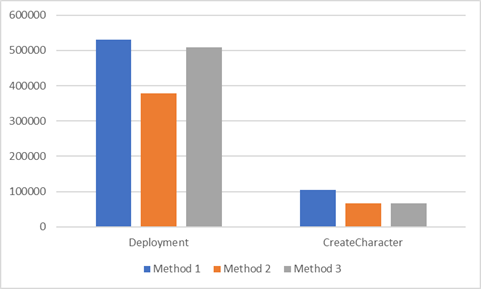
\includegraphics[width=\textwidth]{comparison_methods}
        \label{fig:gascomp:absolute}
    \end{subfigure}

    \hspace{1cm}

    \begin{subfigure}[c]{0.58\textwidth}
        \centering
        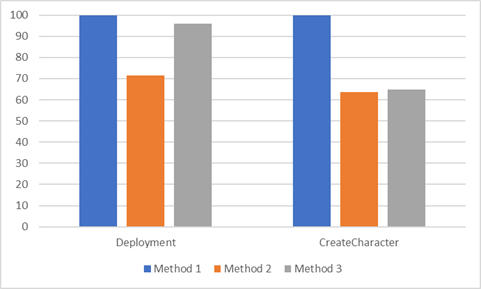
\includegraphics[width=\textwidth]{comparison_methods_pct}
        \label{fig:gascomp:pct}
    \end{subfigure}
    }
    \caption{Gas cost comparison between the 3 proposed methods.}
    \label{fig:gascomp}
\end{figure}

It is clear that the biggest savings are achieved through Method 2. Deploying a contract with Method 2 is 29\% more efficient than Method 1, while Method 3 is only 4\% more efficient than Method 1. Calling \texttt{CreateCharacter} is approximately 36\% more efficient in both methods compared to Method 1. 

Method 2 is the most efficient in terms of gas, however the coding style used for it is extremely compact and non-verbose, which makes difficult to maintain and modify the code, in case software requirements change, as seen in \ref{fig:method2}. In addition, there is no measure taken for overflows, so in case the \texttt{CreateCharacter} function gets called with an argument that is larger than the designed size, the result is miscalculated. 

In an attempt to improve the readability and maintainability of the method by extracting the bit shifting logic to functions the deployment gains over Method 3 are in the range of 5\%, and the function costs differ in the range of 0.001\%, thus negating most of the gas efficiency advantages.

\begin{figure}[ht!]
    \makebox[\linewidth][c]{%
    \begin{subfigure}[b]{0.58\textwidth}
        \centering
        \lstinputlisting[language=Solidity, firstline=1, lastline=9]{contracts/CreateCharacter.sol}
        \caption{Method 1: CreateCharacter}
        \label{fig:method1:createcharacter}
    \end{subfigure}

    \hspace{1cm}

    \begin{subfigure}[b]{0.6\textwidth}
        \centering
        \lstinputlisting[language=Solidity, firstline=29, lastline=39]{contracts/CreateCharacter.sol}
        \caption{Method 1: GetCharacterStats}
        \label{fig:method1:getcharacterstats}
    \end{subfigure}
    }
    \caption{Method 1 \texttt{CreateCharacter} and \texttt{GetCharacterStats} API}
    \label{fig:method1}
\end{figure}

On the other hand, comparing Method 3 (Figure \ref{fig:method3}) with Method 1 (Figure \ref{fig:method1}), they have very similar syntax, with Method 1 being much more efficient in terms of gas. In addition, the bit shifting logic is extracted in a library which makes the code fully portable. Finally, there is more flexibility when performing bit operations due to the usage of \texttt{bytes32} in the library and as a result there is no risk of variables overflowing, contrary to Method 2.

% similar gas efficiency when it comes to calling \texttt{CreateCharacter}. The increased deployment costs happen because it utilizes the \texttt{CharacterLib}, described in \ref{apx:scalability:lib}


\begin{figure}[ht!]
    \makebox[\linewidth][c]{%
    \begin{subfigure}[b]{0.58\textwidth}
        \centering
        \lstinputlisting[language=Solidity, firstline=20, lastline=27]{contracts/CreateCharacter.sol}
        \caption{Method 3: CreateCharacter}
        \label{fig:method3:createcharacter}
    \end{subfigure}

    \hspace{1cm}

    \begin{subfigure}[b]{0.5\textwidth}
        \centering
        \lstinputlisting[language=Solidity, firstline=52, lastline=62]{contracts/CreateCharacter.sol}
        \caption{Method 3: GetCharacterStats}
        \label{fig:method3:getcharacterstats}
    \end{subfigure}
    }
    \caption{Method 3, although similar in coding style, is 36\% more efficient than Method 1.}
    \label{fig:method3}

\end{figure}

In order to effectively compare and evaluate which method is the most effective for the described use case, we evaluate on a weighted score based on \textit{Code Readability}, \textit{Portability}, \textit{Gas Efficiency} o\textit{Security}, as illustrated in Table \ref{table:weights}.

\begin{table}[H]
	\centering
	\vspace*{-1ex}
	\scriptsize
	\vspace{-1ex}
	\begin{tabular}{|c|c|c|}
        \hline
        \textbf{Name} & \textbf{Weight}  & \textbf{Description}\\ \hline 
        Readability/Maintainability & 0.25 & How readable is the codes\\
        Portability & 0.2 & How easy is it to use the code in another smart contract? \\
        Gas Efficiency & 0.3 & How gas efficient is the code? \\
        Security & 0.25 & How robust and secure is the code? \\
        \hline
    \end{tabular}
	\caption{Selected weights for evaluation criteria on picking the most effective method.}
    \label{table:weights}
\end{table}

The result of the evaluation is shown in Table \ref{table:evaluation}:

\begin{table}[H]
	\centering
	\vspace*{-1ex}
	\scriptsize
	\vspace{-1ex}
	\begin{tabular}{|c|c|c|c|c|c|c|c|c|}
        \hline
        \textbf{Name} & \textbf{Weight}  
      & \textbf{M1} & \textbf{M1 (W)}
      & \textbf{M2} & \textbf{M2 (W)} 
      & \textbf{M3} & \textbf{M3 (W)}\\ 
        \hline 
        \textbf{Readability/Maintainability} & 0.3 & 5 & 0.15 & 2 & 0.2 & 3 & 0.3\\
        \textbf{Portability} & 0.3 & 5 & 0.15 & 2 & 0.2 & 3 & 0.3\\
        \textbf{Gas Efficiency} & 0.3 & 5 & 0.15 & 2 & 0.2 & 3 & 0.3\\
        \textbf{Security} & 0.3 & 5 & 0.15 & 2 & 0.2 & 3 & 0.3\\
        \hline
        \textbf{Total} & 0.3 & 5 & 0.15 & 2 & 0.2 & 3 & 0.3\\
        \hline
    \end{tabular}
	\caption{Evaluation for each method based on the criteria from Table \ref{table:weights}. Columns with (W) contain the weighted score for each criterion.}
    \label{table:evaluation}
\end{table}


Taking the above into consideration, we choose to use Method 3 in order to make the implementation described in Chapter \ref{ch:implementation} more gas efficient while retaining its readability and maintainability.

% In Method 1 (\ref{table:tightpacking}) the optimizer is able to cut down deployment costs by 42\%, due to being able to pack all variables in a storage slot. 

% In Method 2 (\ref{table:uint_masking_gas}), the optimization is done manually and has significant results both in deployment and in function costs. In Method 3 (\ref{table:byte_masking_gas}), although we follow the same pattern as in Method 2, we introduce a more verbose API which results in more complex operations being done at a lower level. This introduces slightly bigger deployment costs, and a negligible difference in gas costs for function calls. We consider this overhead to be worth it, since we export an API that is usable.



% Deciding how many times to run the optimizer requires estimating the expected usage of the smart contracts. Comparing the results from running the optimizer 1 and 500 times in Method 2, it can be seen that the deployment costs can increase by as much as 10\% while the savings for each function call are in the range of 0.7\%. When quantifying these percentages in gas, we conclude that if a function is going to be called \textit{enough}\footnote{Enough is not quantifiable and depends on the implementation. A developer should perform a similar analysis to the one we do in order to set their breakeven points.} times, then the contract which was compiled with more optimizer runs is more efficient in the long run. In addition, this shifts the costs towards the contract deployer rather than the users. Given the tradeoffs described above and the improved code readability and maintainability, we opt to use Method 3 in our implementations. 

% Depending on how many times the optimizer is run, there is a different breakeven point for making it worth running more than one times. Running the optimizer 100 times requires the `CreateCharacter' function to be called at least 24 times to make it worth it. % EXPLAIN BETTER THE QUANTIFICATION OF THE TRADEOFF PER FUNCTION CALL COMPARED TO DEPLOYMENT COSTS. Also, the initial cost comes on deployment from the deployer side 
% Even though 1300 gas at the price of 20gwei translates to 0.0000299 https://ethgasstation.info/calculatorTxV.php, this can be a considerable amount considering that a funciton call in a decentralized future might be called millions of times. 1 

% In addition, as we essentially do the optimization ourselves, the deployed bytecode is smaller. 
% This is not exactly intuitive, as it'd be expected that the solidity compiler is able to pack everything perfectly. this method is far more efficient. With this method we are able to store and fetch all the data in a very efficient way, which costs X\% gas less than the previous implementation. However, this method does not allow for a readable and maintainable interface. In order to export every functionality it is needed to convert the `uint' variables to bytes to perform the bit operations on functions. This creates undesired overhead and thus is avoided.

%We described a technique which relies on the compiler's optimizer to pack the data in a struct and do the gas savings, however is simpler and more elegant. The second and third technique are more complex and allow for further gas optimizations. The second technique is more efficient however lacks reusability and is less maintaneable. On the other hand, utilizing libraries however we can export a user-friendly API for reusing our code for anyone who has the same use case as us. This technique will be utilized in the Design and implementation section.
\chapter{Ethereum and Security} \label{security}

The Ethereum platform itself has proven to be robust and reliable as a blockchain as it has been resistant to both censorship and double-spend attacks. In this chapter we discuss vulnerabilities that have been found in the network's implementation which resulted in Denial of Service-like attacks and the blockchain's state being bloated with junk data. Afterwards, we discuss the security of smart contracts and the best practices that need to be applied in order to have a proper workflow. We contribute to the existing literature by evaluating the usage of the tool `Slither' towards finding smart contract vulnerabilities and edge cases. We also improved `Slither' by augmenting the scope of vulnerabilities it was able to detect.

\section{Past Attacks}
\subsection{Network Level Attacks}

\paragraph{October 2016 Spam Attacks}
During the period of September-October 2016, an attacker was able to spam the Ethereum network's state by creating 19 million `dead' accounts. The attack was made possible by a mispricing in the SUICIDE opcode of smart contracts, allowing an attacker to submit transactions that created new accounts at a low cost. The creation of these accounts filled the blockchain's state with useless data which resulted in clients being unable to synchronize in time, effectively causing a \textit{Denial of Service} attack to the network \cite{eip150faq}. As a response, two hard-forks\footnote{A non-backwards compatible upgrade mechanism that creates new rules for a blockchain, usually to improve the system} were proposed \cite{eip607, eip608}. Tangerine Whistle\footnote{EIP608} solved the gas pricing issue and at a later point, Spurious Dragon\footnote{EIP607} cleared the world state from the accounts created by the attack. 

\paragraph{Eclipse Attacks on Ethereum}
\cite{cryptoeprint:2018:236} describes \textit{Eclipse} attacks on Ethereum, a type of attack which by flooding a node's TCP connections is able to make them see a different blockchain history than the network's actual one. This was an attack which was known on Bitcoinwhich was considered to be harder to perform on Ethereum nodes. The researchers communicated the potential effects of the attack and the vulnerabilities were fixed in geth v1.8\footnote{Most popular implementation of Ethereum in golang}. This vulnerability was not abused in the wild, and as a result there was no need for a hard-fork. It should be noted, that other client implementations such as parity or cpp-ethereum were not found to be vulnerable, which shows that having a diverse set of implementations of a protocol can contribute to the network's security.

\subsection{Smart Contract Attacks}
Contrary to the network itself, Smart Contracts have proven to be quite vulnerable in the past. We proceed to give a brief description and explanation of the three biggest hacks in Ethereum's Smart Contracts, involving the TheDAO and a multisignature wallet implementation by Parity Technologies\footnote{\url{https://www.parity.io/}}.

\subsubsection{TheDAO}
TheDAO is an acronym for The Decentralized Autonomous Organization. The goal of TheDAO was to create a decentralized business where token holders would vote on porjects to get funded. TheDAO was initially crowdfunded with approximately \$150.000.000, the largest crowdfunding in history, to date. In July 2016 it was proven that the smart contract governing TheDAO was vulnerable to a software exploit which enabled an attacker to steal approximately 3.600.000 ether, worth more than \$50.000.000 at the time.

If a user did not agree with a funding proposal they were able to get their investment back through a \textit{splitDAO} function in the smart contract. The function was vulnerable to a \textit{reentrancy}\footnote{Essentially because an account's balance was not reduced before performing a withdrawal it was possible for a malicious user to perform multiple withdrawals and withdraw bigger amounts than their balance allowed.} attack which allowed an attacker to make unlimited withdrawals from TheDAO contract\cite{bloombergdao,hackingdistibuteddao}.

What made TheDAO hack very significant was that as a response, part of the Ethereum community decided to perform a hard-fork to negate the mass theft of funds. This was not accepted by the whole community, and as a result, nodes which did not decide to follow the hard-fork, stayed on the original unforked chain which is still maintained and is called `Ethereum Classic' \cite{etc}. 

\subsubsection{Parity Multisig 1}
In July 2017 a vulnerability was found in the Parity Multisig Wallet\footnote{A cryptocurrency wallet, in this case a smart contract, which requires more than one cryptographic signatures to perform a transaction. It is generally used in organizations and to decrease the chances of funds being stolen.} which allowed an attacker to steal over 150.000 ether \cite{parityhack}. The attack involved a library contract, which contrary to using Solidity's `Library' pattern discussed in \ref{method3}, it involves using the \textit{proxy libraries} pattern \cite{proxylibraries} to extract the functionality of a smart contract and let it be usable by other contracts, in order to reuse code, and reduce gas costs, as best practices dictate.

The vulnerability in this was that the Library contract involved a \textit{initWallet} function which was being called through the Parity Multisig Wallet. The function was called when the contract was initially deployed in order to set up the owners of the multisig wallet, however due to it being unprotected\footnote{Public or External visibility without any access control.} it was callable by any user of the wallet\footnote{\url{https://github.com/paritytech/parity/blob/4d08e7b0aec46443bf26547b17d10cb302672835/js/src/contracts/snippets/enhanced-wallet.sol}}. As a result, a malicious user could reinitialize any multisig with their addresss as the contract's owner and drain its funds.

This was observed by a group of hackers called the `White-Hat Group' who proceeded to drain vulnerable wallets before the attacker could, saving more than \$85.000.000 worth of ether at the time. The unrestricted usage of \textit{delegatecall} as well as the lack of proper access control on the \textit{initWallet} function was the root of this hack. 

\subsubsection{Parity Multisig 2}
After the first Parity hack, a new multisig wallet library was deployed, with the visibility in the \textit{initWallet} function initialized. This provided the expected functionality to all Parity Multisig implementations which were using the library. The fix in \textit{initWallet} involved adding \textit{only\_uninitialized} modifier which would only allow modification of the linked multisig's wallet owners during initialization. However, the library itself was not ever initialized. As a result, any user could call the \textit{initWallet} function and set themselves as the owner of the library contract. This alone would not have been dangerous, had there not been a \textit{kill} function in the smart contract, which when called deletes the contract's bytecode, and effectively renders it useless. 

The attacker first\footnote{Although claiming they were not aware of their actions' consequences} became owner of the library by calling \textit{initWallet} with their address as argument, and then proceeded to kill the library. This resulted in \textbf{all} contracts that were using the library's logic to be rendered useless, effectively \textit{freezing} 513774 Ether, as well as tokens \cite{paritypostmortem}. 

A number of proposals were made \cite{eip867} in order to recover the locked funds. All of these would require an `irregular state change' similar to what happened with the DAO\footnote{~12 million ETH were moved from the “Dark DAO” and “Whitehat DAO” contracts into the WithdrawDAO recovery contract\cite{daofork2}} which was eventually dismissed. 

% https://github.com/paritytech/parity/issues/6995
\section{Evaluating Smart Contract Security}
Due to the high financial amounts often involved with smart contracts, security audits from internal and external parties are considered a needed step before deployment to production. It is also being practiced that companies with public smart contracts also engage in bug-bounties, where they encourage users to interact with versions of their contracts deployed on a testnet, in order to identify any other vulnerabilities. Comprehensive studies on identifying the security, privacy and scalability of smart contracts \cite{DBLP:journals/corr/abs-1710-06372} as well as taxonomies aiming to organize past smart contract vulnerabilities have been done \cite{Atzei:2017:SAE:3080353.3080363,tools} have been done, however due to the rapid evolution of the field they get outdated very soon. 

There is a need for auditors and developers to use automated auditing tools on their smart contracts and also use the latest version of the Solidity  Compiler. As an example, none of the tools mentioned in \cite{tools} were able to detect the `Uninitialized Storage Pointer' vulnerability\footnote{\url{https://github.com/ethereum/solidity/issues/2628}. This particular vulnerability has been exploited in Smart Contract honeypots as discussed in Section X}, however the Solidity Compiler was later updated to throw a Warning if this vulnerability exists. 

\subsection{Automated Tools}\label{slither}

Auditing smart contracts significantly more effective when the source code is available. Taking into account the tools which have not been examined in our literature, we came in contact with TrailOfBits, a security auditing firm, and used their suite of tools to extend the already built taxonomies.

We utilized the tool Slither\footnote{Currently not open-sourced. TrailOfBits shared it with us to use it in the thesis.} to audit smart contracts which had their source code available. As our concern is primarily in auditing and ensuring smart contracts that have yet to be deployed, we process all the smart contracts with the latest version of the Solidity compiler, v0.4.21, which provides verbose warnings and errors. 

As Slither is a static analyzer and works on the source code, its modules (called `detectors') are to find certain coding patterns which can be considered harmful to the smart contract. This includes detecting popular past contract vulnerabilities such as Reentrancy or the `Parity bugs', however it's not limited to that. New functionalities can be added through its scriptable API. We describe its modules:

\textbf{Constant/View functions that write to state:} It is planned to make constant and view functions unable to modify state variables by default in the next Solidity compiler versions, however until that happens, it should be enforced manually by developers. It ensures that the code functions as advertised.

\textbf{Misnamed constructors that allow modification of `owner'-like variables:} A constructor in a smart contract is run once at contract creation and usually sets an `owner' variable which allows the contract's deployer to have some extra functionality on the contract. In past cases, constructors were not named properly and were callable by adversaries, leading to smart contracts being drained of funds \cite{Atzei:2017:SAE:3080353.3080363}

\textbf{Reentrancy bugs:} After TheDAO brought reentrancy and race-to-empty\footnote{\url{http://vessenes.com/more-ethereum-attacks-race-to-empty-is-the-real-deal/}} to the spotlight, all vulnerability scanners for Ethereum smart contracts are able to detect this vulnerability.

\textbf{Deletion of struct with mapping}: Deleting a struct with a mapping inside resets the contents of the struct, however it does not clear the contents of a mapping. This has not been reported as an exploit in the wild\footnote{TrailOfBits have found this bug in audits}, however it can be critical in the case of a banking DApp that keeps tracks of balances. A full Proof of Concept is given Appendix A. % TODO

\textbf{Variable Shadowing:} This is a unique feature of Slither that has not been implemented in other scanners (has been used in honeypot contracts).

\textbf{Similar Naming between Variables:} Warns users in the case two variables with same length have very similar names. This is used to have more clear variable naming in order to avoid misconceptions and typos.

\textbf{Unimplemented Function Detection:} This ensures that the implementation of an interface stays compliant and does not diverge from the intended specification.

\textbf{Unused State Variables:} Detects state variables that are not used in any operations and suggests their removal.

\textbf{Unprotected Function Detection:} Detects public functions which have no modifiers and do not perform any assertions on state variables. The current implementation can impose false positives, however it does not have false negatives. This is able to find the Parity Wallet hack.

\textbf{Wrong Event Prefix:} As per the best practices, the names of `events' should be capitalized. After a discussion on Github\footnote{\url{https://github.com/ethereum/solidity/issues/2877}}, using `emit' for events is going to be a mandatory for Solidity 0.5.0 and onwards.

It is seen that Slither can be used both for finding known vulnerabilities, but also to avoid common coding anti-patterns and mistakes. Due to its highly scriptable API we can extend it to include more rules. We contributed to the Slither repository by adding support for detecting \textit{tx.origin} and \textit{block.blockhash} usage. The usage of \textit{tx.origin} should be avoided unless necessary, and as stated in the Solidity documentation can incur in loss of funds\footnote{\url{http://solidity.readthedocs.io/en/v0.4.21/security-considerations.html}}. \textit{block.blockhash} has been misused in smart contracts and ended up in 400 ETH being stolen from a company called SmartBillions \cite{smartbillions}. We also contributed to the improvement of the accuracy of the modules `UnimplementedFunctionDetection'. Figure X shows a comparison of Slither after our contributions to the other analysis tools from \cite{tools}. 

[CREATE GRAPH WITH SLITHER FINDING VULNS SAME AS OTHER TOOLS]

\subsection{Honeypot Smart Contracts}
Since the second Parity bug and as of March 2018, no novel critical vulnerabilities have been identified in smart contracts. However, smart contracts that are architected to look vulnerable to known exploits started surfacing, when their true purpose is stealing the funds of aspiring hackers. These contract honeypots are funded with an initial small amount of ether (0.5 to 2 ether). Hackers who attempt to exploit them need to first deposit some amount (depending on the honeypot's implementation) before trying to drain the contract. Each honeypot has a well-hidden mechanism to prevent the attacker from draining the funds, essentially locking up any funds that get deposited by individuals other than the contracts deployer. 

\begin{figure}[H]
    \centering
    \lstinputlisting[language=Solidity]{code/Gift_1_ETH.sol}
    \caption{Example honeypot}
    \label{smart_contract}
\end{figure}

The above contract was initialized with 1 ether at its balance. An attack can drain the contract by calling the $GetGift$ function with the correct password. Due to the attacker not knowing the password, they proceed to change it, using the $SetPass$ function, which requires at least a 1 ether deposit, which is acceptable since the attacker will get that back. This also requires that the `passHasBeenSet' variable is false, or that the PassHasBeenSet function has not been called yet.

A naive attacker would inspect the contract's transactions in Etherscan\footnote{https://etherscan.io/address/0xd8993f49f372bb014fb088eabec95cfdc795cbf6} and after notice that no transaction refering to `PassHasBeenSet' has been made, and thus proceed to attack the contract and change the password, only to find that the password did not get changed. A transaction where a contract calls another contract's function is called a `Message Call'. Etherscan shows this kind of calls as `Internal Transactions', only when they include values of more than 0 ether. In this case, `PassHasBeenSet' does not accept Ether and thus cannot be detected in Etherscan. The contract's owner called `PassHasBeenSet' from another contract and as a result the password is not changeable. Detecting that the `passHasBeenSet' variable had been set to true can be done by inspecting the storage of the smart contract, which is always public as shown in \ref{fig:storage}

An extensive analysis of smart contracts as honeypots is made in \cite{honeypots} which was released to accompany the research of this Master Thesis.


\subsection{Towards more secure smart contracts}
It is apparent that since smart contracts being unmodifiable after deployment, there is no way of patching any vulnerabilities. Testing platforms have been setup so that developers can practice and test their skills. A developer should keep their code as simple as possible, while providing test coverage for as many scenarios as possible. Using audited and tested code for parts of contracts that have already been implemented (eg. an $ERC20$ token contract) ensures that these parts of the code are going to be secured. Following the best practices as described by the industry\'s most sophisticated auditors\footnote{\url{https://consensys.github.io/smart-contract-best-practices/known_attacks/}}. Finally, developers should be looking for confluence between the results of different automated analyzers in order to filter out false-positives and find false-negatives.
% % https://ethernaut.zeppelin.solutions/
% % http://hackthiscontract.io/
% http://solidity.readthedocs.io/en/v0.4.21/security-considerations.html#recommendations
\chapter{Metering and Billing of Energy on Ethereum}\label{ch:implementation}

Smart contracts can transform the energy industry. In this chapter we explore the inefficiencies of the energy market and identify gaps which can be filled by blockchain. We go through the advantages of an energy-based application built on smart contracts. Finally, we describe the business logic of a specific energy use-case which we implemented on Ethereum. The implementation takes into account the methods and concepts described in Chapter \ref{ch:scalability} and Chapter \ref{ch:security} in order to ensure that the smart contracts are efficient and robust.


\section{Energy Market inefficiencies}

The global energy market is gradually transitioning to clean and renewable energy. Regulations encourage usage of distributed energy resources (DERs) \cite{europe2030}. With the integration of DERs, consumers are gradually transforming to \textit{prosumers} who store their energy surplus or sell it to their peers, effectively distributing the generation of energy, contrary to existing power systems which were designed to accommodate central points of energy generation.

There are numerous inefficiencies which need to be resolved in today's energy markets~\cite{ey-inefficiencies}:
\begin{enumerate}
    \item \textbf{Transaction complexity:} More participants in the networks result in more complex transactions.
    \item \textbf{Predictability and Reliability:} Availability of DERs is less predictable compared to traditional energy resources like coal. 
    \item \textbf{Empowered prosumer:} There need be monitoring tools and infrastructure that allow prosumers to manage their energy production and consumption.
    \item \textbf{Geographic mismatches:} Locations that fully utilize DERs are usually far from key points of energy demand. Transmitting energy over long distances is inefficient.
    \item \textbf{Trust and Security:} New participants will only choose the system if it is able to be trusted and is properly secured.
\end{enumerate}

%Today's energy markets are called to resolve a number of issues.
% Having discussed how Ethereum works, and explained techniques to improve smart contracts' scalability and security, we proceed to discuss the topic of making energy markets more transparent and efficient by utilizing smart contracts. The use-case we describe can be used as a starting point for better tracking of energy usage inside a company, allowing better prediction of future needs.  
% The world is gradually shifting from nuclear and fossil fuels to Renewable Energy Sources (RES). RES have been taking a larger share of Germany's gross energy production and this has created a 
% Germany is on a rollout plan of installing smart meters in every household which incorporates RES.  
% The barrier to entry to become an energy producer\footnote{By installing solar panels for example} 
% Chart for renewables: https://www.cleanenergywire.org/factsheets/germanys-energy-consumption-and-power-mix-charts
% In its current state, most consumers do not know what they are paying Business level take long time and are 

% Price of energy, consumer does not know always what they pay, or what they gain from their renewables
 
\section{Energy Market use-cases for Blockchain}

A number of use-cases for smart contracts have been identified in the energy market. We proceed to describe applications that derive from the advantages of blockchain (transparency, trustlessness, security) as discussed in Section~\ref{advantages}.

\begin{enumerate}
    \item \textbf{Supply chain tracking and optimization:} This is a broad blockchain use case which allows for optimization on logistics and tracking the location of products, reducing fraud and ensuring the validity of an event.
    \item \textbf{Energy metering and billing:} By committing the values of energy consumed by entities to a blockchain, a timestamped record of meter readings gets generated which allows for the verification and more clear understanding of energy consumption across resources. This can be augmented to provide billing functionality (further described in \ref{business-logic}).
    \item \textbf{Peer to Peer (P2P) energy trading:} Consumers and prosumers operate in a local microgrid and trade energy between them, without a centralized operator, resulting in reduced loss of energy during transportation.
    \item \textbf{P2P Energy Micropayments:} A car that is far from its charging station is charged by the surplus energy of another car. Since this is a short-lived process that happens often, such as during the waiting time at a traffic light, in order to send and receive micropayments between the involved parties, a blockchain can be used to utilize fast payments and low transaction fees. 
    % It can also contribute to peak shaving~\footnote{Energy is billed based on the peak energy consumed during a time window. By consuming energy for charging during low peak times the peak can be reduced.} effectively reducing the costs during that time window.
\end{enumerate}

% By using smart contracts, all of the above use-cases can be automated
% Use Cases:
% - P2P Energy Trading
% - Sharing Economy - EV share and charge

% Internet of Things sensors can securely streamline inspections and repairs and automatically reduce outages.
% Applications have been developed \cite{DBLP:journals/ife/MengelkampNBDW18}

% Blockchains have the ability to provide transparency and immutability. Also,  When talking about energy and transparency, full history of meter readings, price calculation, billing of inhouse energy departments. This can be extended for EV car payment microtransactions and so on.

% The blockchain is a particularly interesting technology for decentralized processes that require large networks and trust relationships between all parties. Therefore, it offers great benefits to the power & utilities market, with its large networks of power and utilities companies, (maintenance) subtractors, (local) suppliers and end users.

% Smart meters Still, there are other applications that are ready for use in the near future. Smart meters for instance have already entered many homes. Up until now, sharing data through smart meters was a threat to the privacy of the owner of the meter. Again, the blockchain offers a potential solution. It can provide the accurate data to the supplier without requiring a direct link to the meter of specific users. When needed, the owner of the smart meter can prove to the supplier that the data are his, using his private key, and the cryptographic security of the blockchain proves that the information is accurate and hasn’t been tampered with. This puts the owner in control of his own data.

\section{Business Logic} \label{business-logic}
In collaboration with Honda R\&D Germany, we create a pilot suite of smart contracts for in-house use in order to track and bill the consumed energy of the company's headquarters as measured by a set of smart meters. 

We proceed to discuss the business logic of the use-case and then implement it. We utilize the Method 3 from Section \ref{method3} to optimize our smart contracts for gas efficiency, and utilize Slither from Section~\ref{slither} and the learned best-practices to ensure that the developed smart contracts are robust. The contracts were tested and deployed on a private Ethereum blockchain, however it is possible to deploy the implementation to the Ethereum mainnet.

%The purpose is to serve as a means of tracking the energy consumed by the company's smart meters and ensuring the data's validity and existence in a smart contract. In addition, due to the complex structure of the company, every smart meter's consumption can contribute with different coefficients to the total energy consumption of the rooms in a building. As a result, the developed smart contract are able to track the energy consumption of each room and assign it to a higher-order 

\subsection{Metering of Energy} \label{metering}

\paragraph{Smart Meters}

A smart meter is an energy meter which logs its measured energy readings to a monitoring server. A smart contract must track each smart meter by a unique identifier and store its power readings, along with the corresponding time of measurement. Due to the meter not being able to \textit{ping}\footnote{Hereafter, refers to a kWh,timestamp tuple which gets stored in the blockchain.} its reading directly to the blockchain, we create a pipeline where the reading and timestamp of each meter is pulled from the monitoring server and then pushed to the blockchain. 

\begin{figure}[ht!]
    \centering
    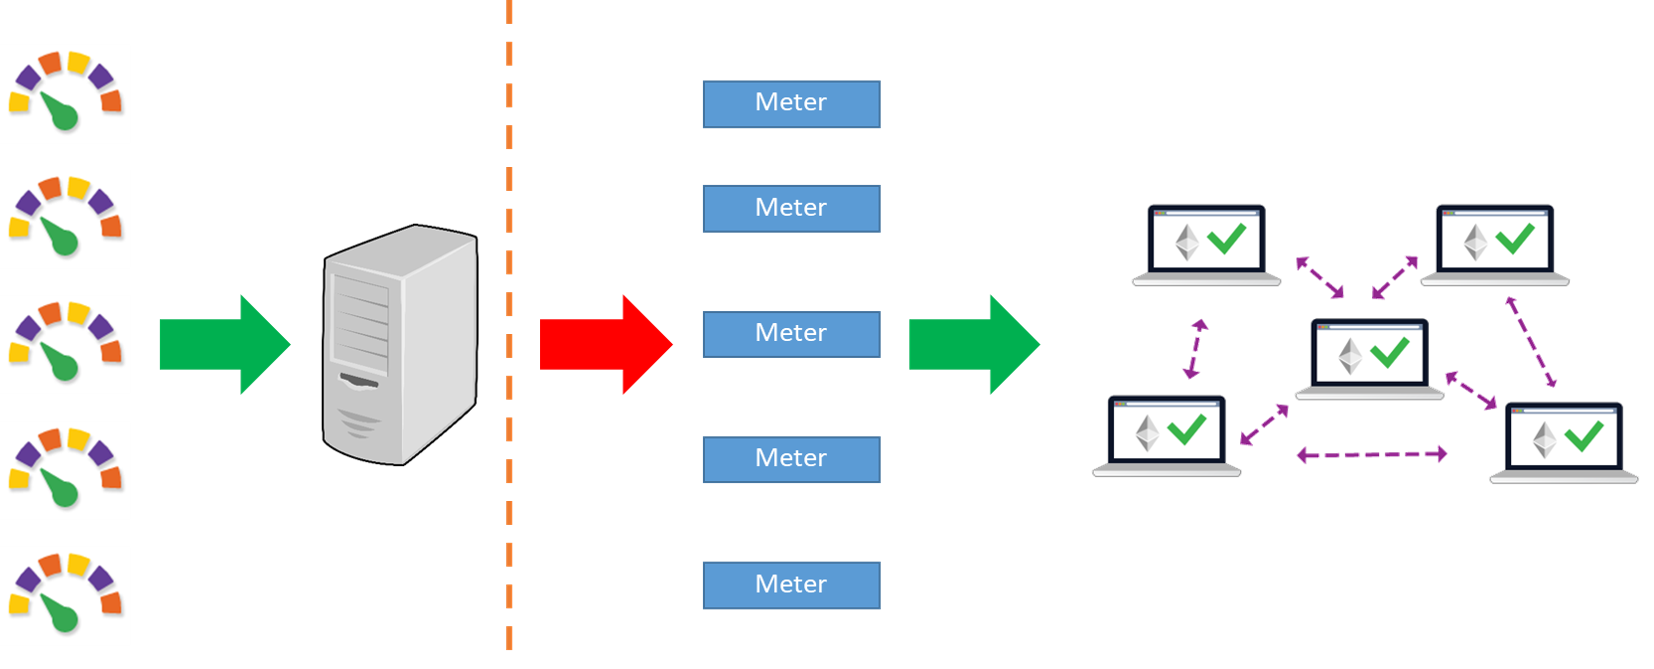
\includegraphics[width=\textwidth]{pull_push_monitoringserver}
    \caption{Meter Data gets pushed to the blockchain after getting pulled from the monitoring server}
    \label{fig:pull_push_monitoringserver}
\end{figure}
% must be able to keep track of the current reading and timestamp of the reading as well as the last reading and timestamp in order to calculate the difference of the two. It also has a unique identifier which is used to retrieve it in the smart contract.

\paragraph{Virtual Meters}

A \textit{Virtual Meter} is a group of \textit{Smart meters}. The purpose of a Virtual Meter (VM) is to track the consumption of multiple Smart Meters across various rooms of a company building. The consumption of a VM is a function of the power consumptions of its linked smart meters. 

The formula that describes each Virtual Meter is supplied from an internal partner and is considered to be known. An example formula can be seen in Equation \ref{eq:formula}. Variables prefixed with $VM$ represent Virtual Meters, $ELT$ and $KMZ$ represent Smart Meters and $F$ represent constants.

It is the case that this process could be done entirely on-chain, by creating a smart contract that manages virtual meters separately. This would require another smart contract for virtual meters, which would need to store the Meter IDs for each meter associated to the virtual meter, along with the formula that describes how the virtual meter consumption is calculated. This logic is unnecessarily complex to be performed on a smart contract directly. Instead, it is done off-chain on the client side, by pulling the readings of each smart meter, calculating the reading of the virtual meter, and then pushing the aggregated reading to the smart contract's storage.

\begin{equation} \label{eq:formula}
    \begin{aligned}
        VM15= \\
        & (ELT46-(ELT31+ELT16+ELT17+ELT35+ELT36))*F57
        \\
        + & (ELT35+ELT36-ELT18)*F27*F66
        \\
        + & (KMZ6-KMZ5)*(ELT16+ELT17+ELT18+ELT19+ELT20)\\
        & /KMZ2*F27*F66 
    \end{aligned}
\end{equation}

\begin{figure}[htb]
    \centering
    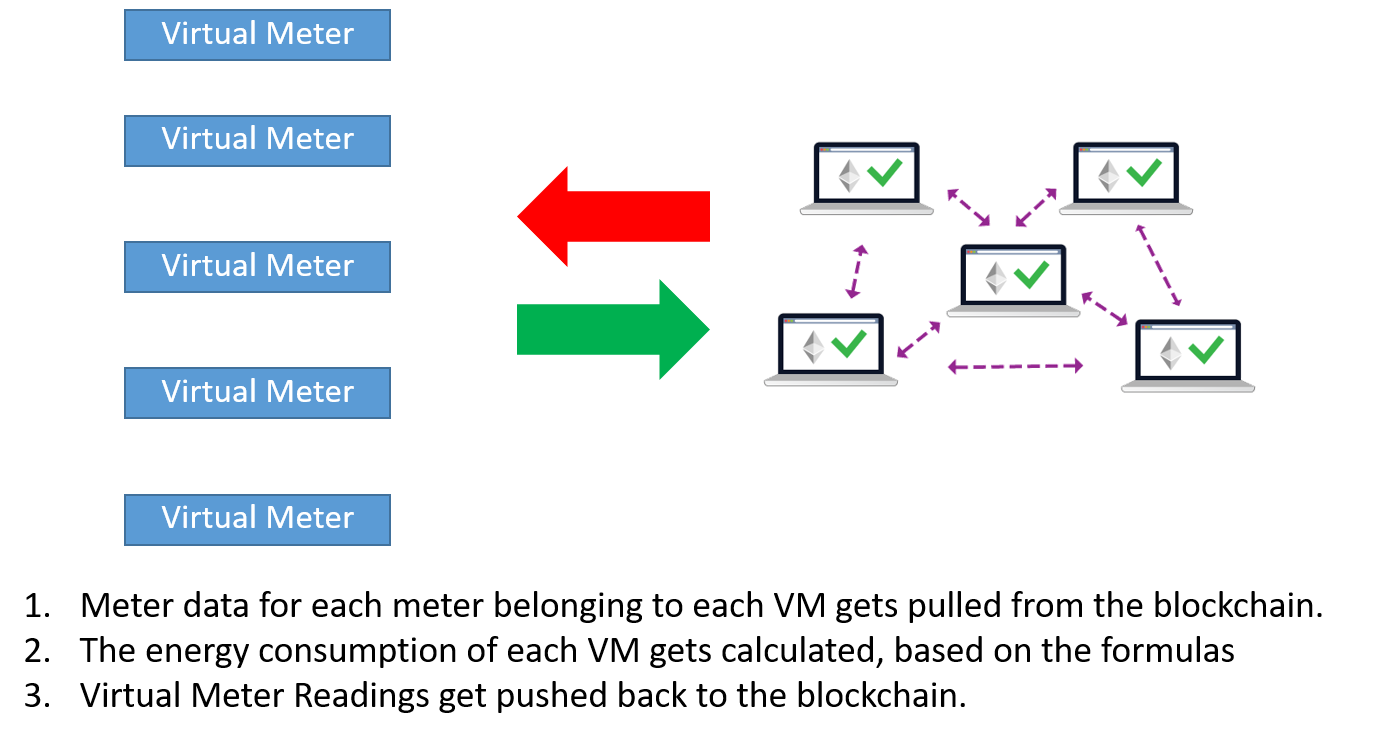
\includegraphics[width=\textwidth]{virtual_meters}
    \caption{The consumption of Virtual Meters gets calculated from the consumption of their associated Smart Meters.}
    \label{fig:virtual_meters_consumption}
\end{figure} % IMPROVE FIGURE

\subsection{Accounting Logic} \label{billing}

The accounting business logic of the company breaks down in a hierarchy which is described by \textit{Business Units} (BUs) and \textit{Departments}. BUs are used for external accounting, while Departments are used for internal accounting. In implementation terms, a Business Unit is equivalent to a Department.

A Department is composed of Virtual Meters, other Departments of a lower tier % better word?
 (hereafter called \textit{Subdepartments}) and \textit{Delegates}. A Department may forward its power consumption to its Delegates as part of the internal accounting process. The total consumption of a department is the sum of energy consumed by its Virtual Meters, Departments and Delegates. After a department delegates its debt, its consumption is considered to be cleared from an accounting perspective.

\begin{figure}[ht!]
    \centering
    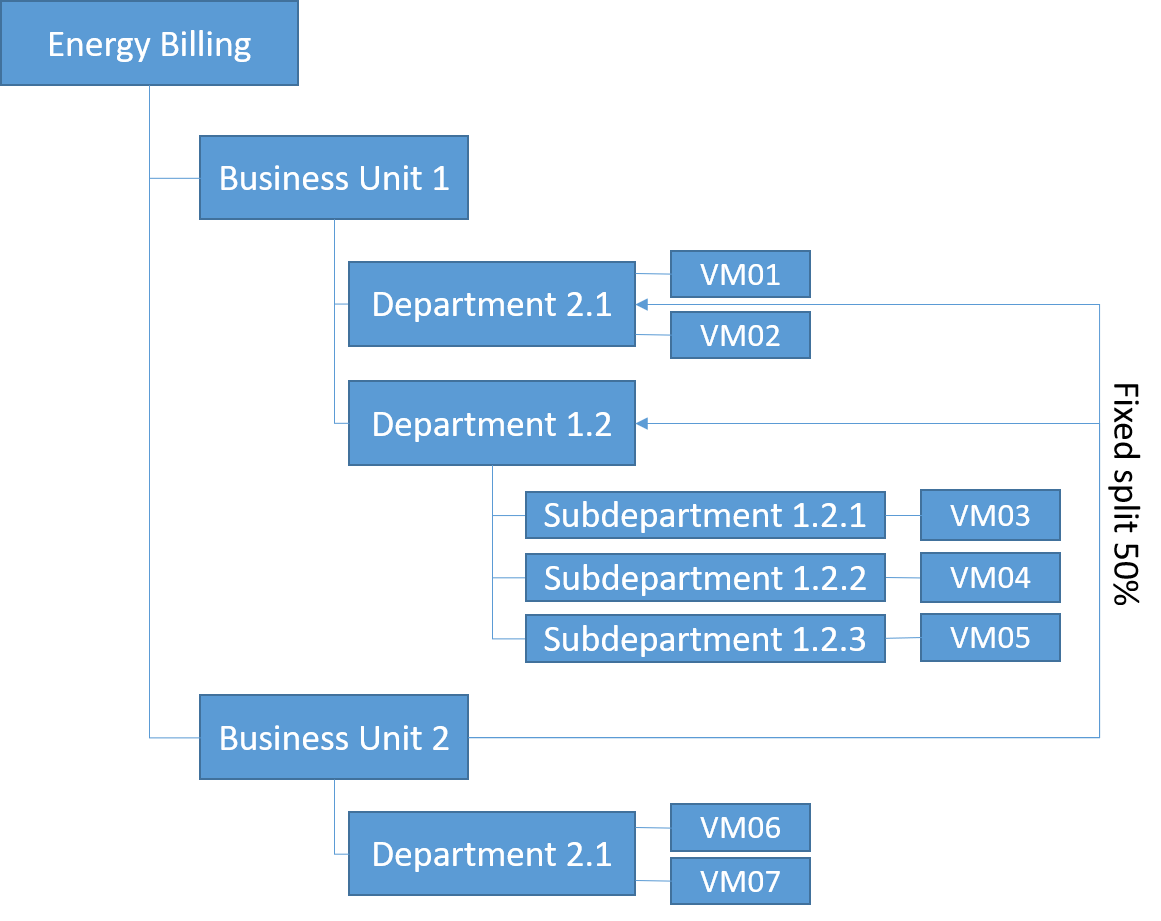
\includegraphics[width=.7\textwidth]{hierarchy}
    \caption{Relationship between Departments and Delegates.}
    \label{fig:hierarchy}
\end{figure} % TODO: BETTER FIGURE

There are two ways for a department to forward its consumption to its delegates:

\begin{enumerate}
    \item \textbf{Headcount Split:} Top tier departments can perform a headcount split of their consumption based on the percentage of staff that works at each \textit{Delegate} department.
    \item \textbf{Fixed Split:} This process can only involve a department which has exactly 2 \textit{Delegates}. The first delegate receives $X\%$ of the sender's consumption and the second delegates receives $(100-X)\%$.
\end{enumerate}

As an example, in \ref{fig:hierarchy} Department 1.1 and 1.2 are fixed split delegates of Business Unit 2. When BU2 forwards its consumption, it will get split among the 2 \textit{Delegates}. After delegation, Business Unit 2 has its consumption cleared and will not be calculated towards the total Energy Billing. The billing process starts from the inner-most tier and iteratively moves outwards until the top-tier departments are reached.


\section{Smart Contracts} \label{ch:implementation:sc}
In this section we go over the implementation and the rationale of each developed smart contract. We explain the inner workings and provide tests of their functionality. We follow the design principle that the data stored on the blockchain is the minimal amount of data that needs to be trustlessly verified. Any piece of data that can be derived from the already on-chain data is generated and verified off-chain. In case data does not need to be accessed by another contract but must be transmitted to an end-user, the \texttt{Event} functionality of Solidity is used (explained in \ref{apx:implementation:events}). 

\subsection{MeterDB}
MeterDB utilizes Method 3 (\ref{method3}) to keep track of the energy consumption values and logged timestamps of a smart meter or a virtual meter. We assume that a meter can be any IoT device that has its own Ethereum account\footnote{As a prerequisite, a private-public keypair needs to be generated for every meter.}. The contract is designed to map each Meter's address to its details (\texttt{id}, \texttt{reading}, \texttt{timestamp}).

The contract is split in two files, \texttt{MeterDB.sol} which contains the business logic, and \texttt{Meter.sol} which contains the gas optimization logic that encodes and decodes meter data in a \texttt{bytes32} variable. In order for a meter to be able to call the \texttt{ping} function it first needs to be activated, by registering its id and address in the smart contract. Deactivating a decommissioned meter results in its data being deleted from the storage of the smart contract, which refunds gas as mentioned in Rule 3 of \ref{ch:scalability}. By storing a mapping of meter ids to address we are able to access a meter's data by id in $O(1)$ instead of iterating over a list of registered meters.

For each meter, its latest reading is pulled from the monitoring server and if a new consumption value has arrived it replaces the previous reading along with its timestamp by calling \texttt{ping}. A \texttt{Pinged} event is emitted after each \texttt{ping} function call which enables users to fetch the full history of readings and timestamps for a meter. Table~\ref{table:meter} illustrates the design of the storage in \texttt{Meter.sol}.

\begin{table}[H]
	\centering
	\vspace*{-1ex}
	\scriptsize
	\vspace{-1ex}
	\caption{Required variables and size to describe a Meter.}
	\begin{tabular}{|c|c|c|}
        \hline
        \textbf{Name} & \textbf{Type}  & \textbf{Comment}\\ \hline 
        meterID      & bytes8         & IDs can be encoded in 8 bytes, can be optimized but hurts UX\\
        creationTime  & uint32         & Meter supports timestamps up to 2**32 = 02/07/2106 @ 6:28am (UTC) \\
        power         & uint32          & Power readings can reach up to 2**32, which is enough to store 1TWh readings \\
        \hline
    \end{tabular}
    \label{table:meter}
\end{table}

\subsection{AccountingDB}

AccountingDB stores the ids of each Virtual Meter, Subdepartment and Delegate in order to be able to calculate the consumption of each Department. 

The setting of energy reading values is done in \texttt{Department.sol} which utilizes Method 3 (\ref{method3}) to keep track of the energy consumed by a department due to its associated Virtual Meters, Subdepartments and Delegates. 

Due to the forwarding of a department consumption to another, we keep track of the power that is generated by the virtual meters, the delegated power that is received from another department, and the cleared power which is the amount of power that has been cleared from that department, either through delegation or from accounting. The consumption forwarding logic is implemented as described in Section~\ref{billing}. A \texttt{active} variable is used to keep track of activated departments.

\begin{table}[H]
	\centering
	\vspace*{-1ex}
	\scriptsize
	\vspace{-1ex}
	\caption{Required variables and size to describe a Meter.}
	\begin{tabular}{|c|c|c|}
        \hline
        \textbf{Name} & \textbf{Type}  & \textbf{Comment}\\ \hline 
        active         & bool         & Department active flag\\
        headcount      & uint7        & Headcount percentage, between 0 and 100\\
        power          & uint80       & Power readings can reach up to 2**80\\
        delegatedPower & uint80       & Power readings can reach up to 2**80\\
        clearedPower   & uint80       & Power readings can reach up to 2**80\\
        \hline
    \end{tabular}
    \label{table:department}
\end{table}

\subsection{Access Control} \label{acl}
As discussed in Chapter \ref{ch:security} enforcing proper access control on critical functions of a smart contract is very important. It is common to find Access Control Lists (ACL) in enterprise environments which allow only participants to access resources based on their clearance levels. This functionality does not exist by default in smart contracts. Access control can be done separately in each contract, by using a whitelist and a function modifier, however that needs to be done for each contract and does not scale for a rich smart contract ecosystem (further explained in \ref{apx:implementation:acl}). 

As a result, we use a pattern for access control by calling a separate smart contract that stores the logic for allowing or denying permission to a user about calling a function of a contract at an address. 

We proceed to describe the access control enforced on each of the actors involved in the developed smart contracts:
\begin{enumerate}
    \item Administrator: Can call all functions in all deployed contracts.
    \item Registry Operator: Can call \texttt{enable} and \texttt{disable} in \texttt{Registry}.
    \item Meter Operator: Can call \texttt{activateMeter} and \texttt{deactivateMeter} in \texttt{MeterDB}.
    \item Accounting Operator: Can call \texttt{activateDepartment}, \texttt{deactivateDepartment} \texttt{setDelegates},\texttt{setVirtualMeters},\texttt{setSubdepartments},   \texttt{setHeadcount}, in \texttt{AccountingDB}.
    \item Accountant: Can call \texttt{billPower}, \texttt{fixedSplit}, \texttt{headcountSplit} and \texttt{clearDepartment} in \texttt{AccountingDB}.
\end{enumerate}

\subsection{Contract Registry} 

In order to be able to retrieve the addresses of smart contracts by name a \texttt{Registry} smart contract was implemented. The contract resolves contract names to addresses through a \texttt{bytes32} to \texttt{address} mapping. The address of a contract can be changed by the registry's operator. This lays the foundation of a basic pattern for upgradeable smart contracts via a controlled name registry. Exploring the possible implementations of upgradeable contracts with this method is considered out of scope for this Thesis. Finally, this method can be utilized in the client scripts in Section \ref{ch:implementation:client} to reduce the number of addresses that need to be supplied to interact with the smart contracts\footnote{The registry's address is provided from the command line and then the registry resolves each contract's address by their names which are known beforehand}.

\subsection{Deployment Pipeline}

The full deployment pipeline involves deploying each contract separately and linking it to the Access Control List as shown in Figure~\ref{fig:pipeline}. At each step, the Administrator grants permissions to call specific functions of the smart contract to each role. Finally, after all contracts have been initialized, their addresses are stored in the Registry for later resolving.


\begin{figure}[htb]
    \centering
    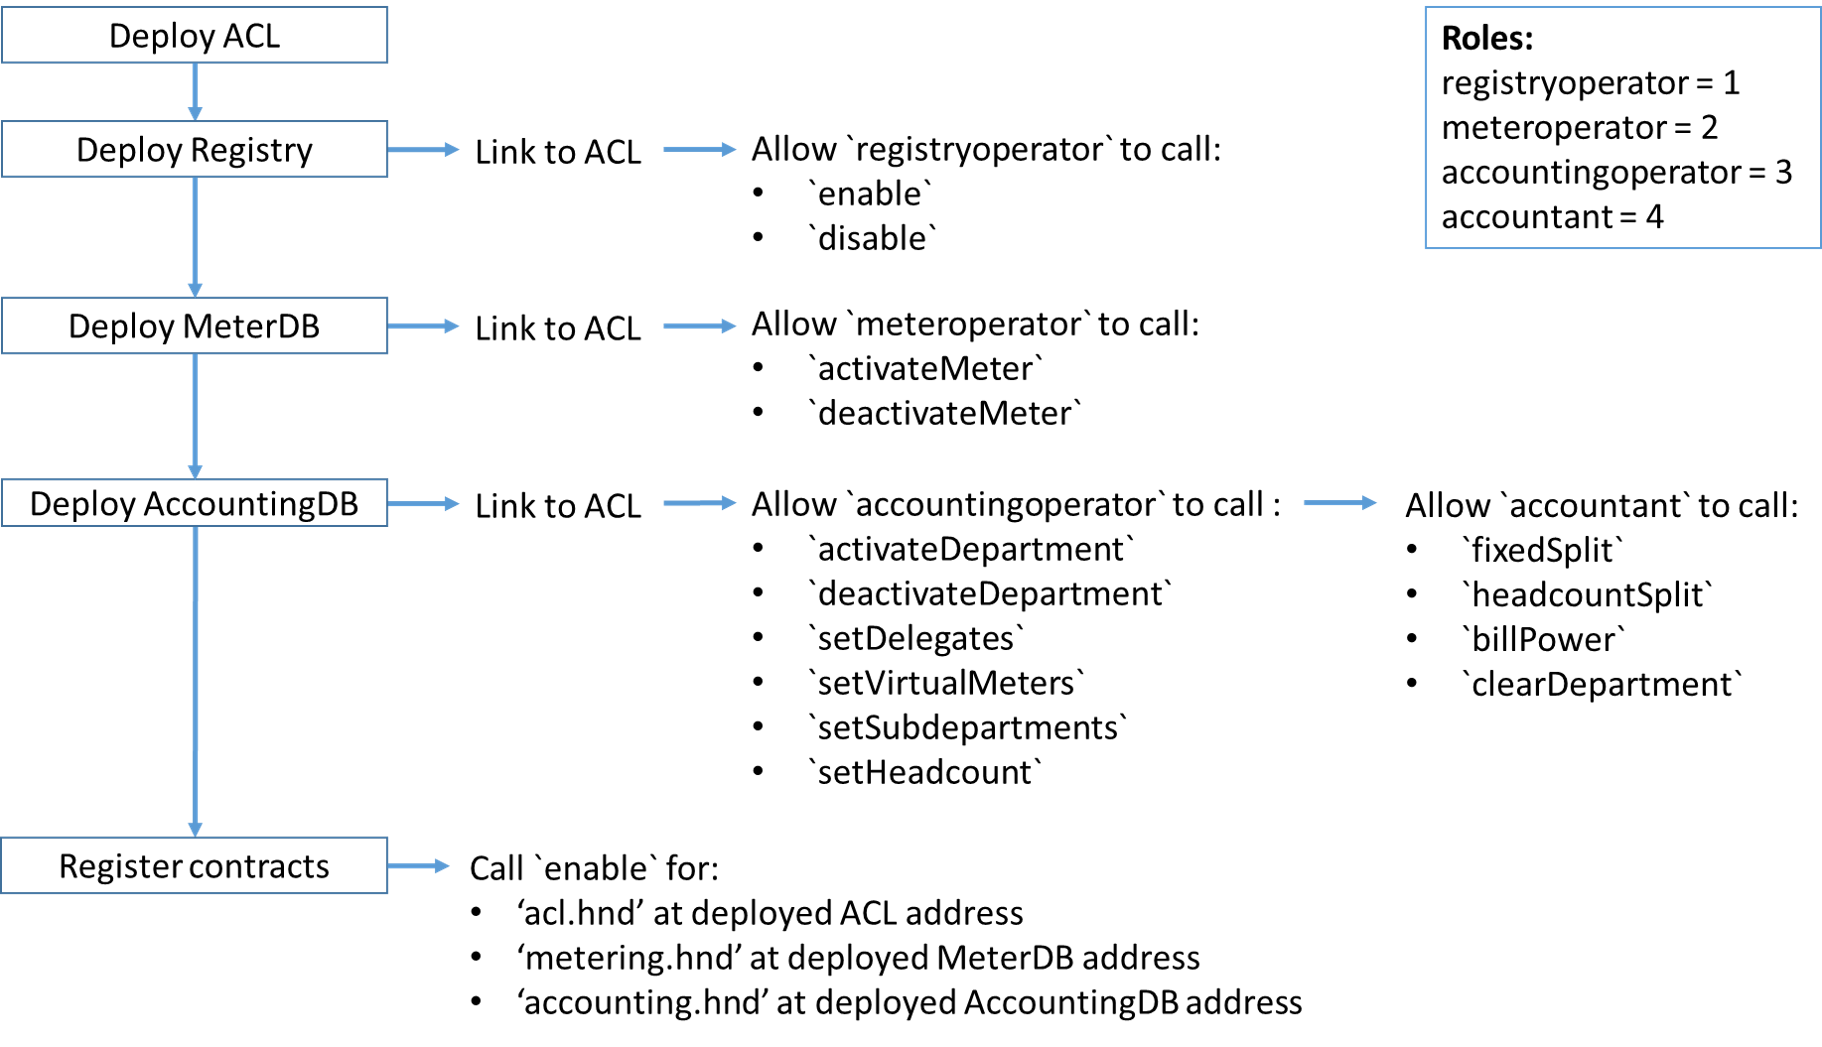
\includegraphics[width=\textwidth]{pipeline}
    \caption{The full deployment pipeline enforcing access control}
    \label{fig:pipeline}
\end{figure}

\section{Client Side} \label{ch:implementation:client}

As described in Section \ref{ch:basics:insideevm}, smart contract functions get executed only in response to transactions made by EOAs. Since the goal is to have an automated process of pulling data from and pushing data to the smart contracts, we implement client scripts which perform that functionality. We use Python and Web3.py to implement utilities and multiple command line interfaces (CLIs) which are used to interact with the smart contracts. A module is also developed for interacting with the REST API of the monitoring server. A separate keypair is generated for every role mentioned in Section \ref{acl}, and each CLI is designed to function only with by using the corresponding role's private key.

% In order to make the code portable and ensure that the clients can be run on any machine, we also provide a Dockerfile. Docker utilizes containerization Due to design, it can be dockerized and run on multiple blabla.

\subsection{Utilities} \label{utils}

\subsubsection*{Web3.py and Contract Wrappers}
We create a wrapper around the web3 library in order to provide a generic interface when connecting to a node. That way, a web3 instance can be return by calling \texttt{getWeb3(endpoint)}. In order to send a transaction, it first must be signed with the sender's private key. In the naive case, the private key can be stored in the node, however the security of this is limited to a user hosting their own node. In the case where multiple clients need to connect to a third-party node, it is a security compromise to host the unencrypted private keys on the node. 

We define a base class called \texttt{Contract} that provides functionality for interacting  with a smart contract. It allows signing and broadcasting of locally signed transactions to a node. It is able to track the nonces of an account separately which means that an account can submit multiple transactions without waiting for the previous one to get confirmed. It receives a compiled contract ABI and address of the corresponding contract, along with a private key for signing the transactions. The exposed function \texttt{sign\_and\_send} is used to specify which function of the contract to call and submit it for execution to an Ethereum node. We use the \texttt{Contract} class throughout our implementation to create user-friendly interfaces for the functions of each contract while maximizing code reusability and security by signing transactions locally.

\subsubsection*{Monitoring Server and Rest API}
As mentioned in Section \ref{metering}, there is no direct access to each meter's reading. As a result, all readings are exposed through an authenticated REST API. We implement a module which gets instantiated with a Meter id as a parameter, and is able to interact with the monitoring server API. The primary function used is \texttt{get\_single\_reading} which fetches 1 reading from the monitoring server, by default the most recent one. Implementing the whole set of functionality provided from the API was considered out of scope becaues it did not provide any additional information for our use-case.

\subsection{Administrator CLI}
The administrator role is used to grant or revoke role permissions to operators. The CLI interacts with the ACL smart contract which has been initialized as described in Section \ref{acl}.  As input, it expects an action (grant, revoke) and a json configuration file with the address of each account and its corresponding role to be granted or revoked. If no configuration file is supplied, it is expected that a role and address is provided as command line arguments. A user can additionally supply the \texttt{fund} parameter to send ether for the gas costs the operators will incur for interacting with their corresponding smart contracts. 

\subsection{Registry Operator CLI}
The registry operator's role is used to enable or disable a contract in the \texttt{Registry} contract. It can be utilized to register a new contract name and address at a later point in time or to remove an existing contract from the listing. The CLI also provides the functionality to resolve a contract name to its address or a contract address to its name. 

\subsection{Meter Operator CLI} \label{meter-operator}
The meter operator role is used to activate or deactivate smart meters in the \texttt{MeterDB} contract. The \texttt{ping} function is decorated with the \texttt{onlyMeter} modifier which requires for a meter to first be activated to successfully call it. As input, it expects a json configuration file with the address of each meter and its id. If no configuration file is supplied, it is expected that an address and a meter id is provided as command line arguments. By providing the \texttt{deactivate} parameter, it instead deactivates the meters. A user can additionally supply the \texttt{fund} parameter to send ether for the gas costs the meters will incur for calling \texttt{ping}.

\subsection{Accounting Operator CLI}
The accounting operator role is used to activate or deactivate departments in the \texttt{AccountingDB} contract. After activation, the operator should set the department's headcount, virtual meters, subdepartments and delegates according to the business logic. As input, the CLI expects a json configuration file which represents the business logic and which functions to be called for each department. 

\subsection{Single and Multiple Meters CLI}
A \texttt{meter} module is implemented which is responsible for connecting to \texttt{MeterDB} and the monitoring server through the API as explained in Section \ref{utils}. The meter first needs to be activated by the meter operator as explained in Section \ref{meter-operator}. The client is responsible for polling the monitoring server. When a new power reading arrives for the meter, it is pinged to the smart contract. The \texttt{single-meter} CLI expects the meter's private key as input, and retrieves the meter id from the smart contract in order to connect to the monitoring server.

Due to having multiple smart meters in our use-case, a \texttt{multiple-meters} CLI is also implemented which is responsible for launching multiple \texttt{single-meter} processes, each one running independently of each other. The output of each process is saved in a timestamped log file.

\subsection{Single and Multiple Virtual Meters CLI}
A \texttt{virtualMeter} module is implemented which is responsible for connecting to \texttt{MeterDB} and pulling the reading of its connected meters as described in Section \ref{metering}. Along with the virtual meter's private key a formula is supplied to the CLI as arguments. The virtual meter and the meters included in the formula must be previously activated by the meter operator. Given the formula, each referenced meter's readings are fetched, and the formula is evaluated\footnote{Using the module: \url{https://github.com/Axiacore/py-expression-eval}} before pinging the final value to the smart contract.

Similarly to normal smart meters, a \texttt{multiple-virtualmeters} CLI is implemented which is responsible for launching multiple \texttt{single-virtualmeter} processes, each one running independently of each other. The output of each process is saved in a timestamped log file.

\subsection{Accountant CLI}
The accountant module is responsible for pulling all the readings associated with a department, calculating the total amount of energy to be billed to the department as well as performing any forwarding of energy to a department's delegates. The accountant is simultaneously connecting to \texttt{MeterDB} and \texttt{AccountingDB}. Even though the accountant role is not authorized to access the functions related to pinging or operating in \texttt{MeterDB}, accessing the data for each meter can be done without supplying the contract instance with a private key\footnote{Viewing data stored in a smart contract is free as it involves directly querying the node for its storage and does not involve any state mutating transaction. As a result, no private key is needed to access the meter readings.} 

The departments are processed in order from the inner-most tiers towards the top level departments, as described in Section~\ref{billing}. The flowchart in Figure \ref{fig:consumption_flowchart} shows the process that each department goes through in order to correctly calculate its final consumption.
% since the consumption of a department may be dependent both on its associated virtual meters, which are stored in \texttt{MeterDB}, and its subdepartments or delegates. The connection 

\begin{figure}[H]
    \centering
    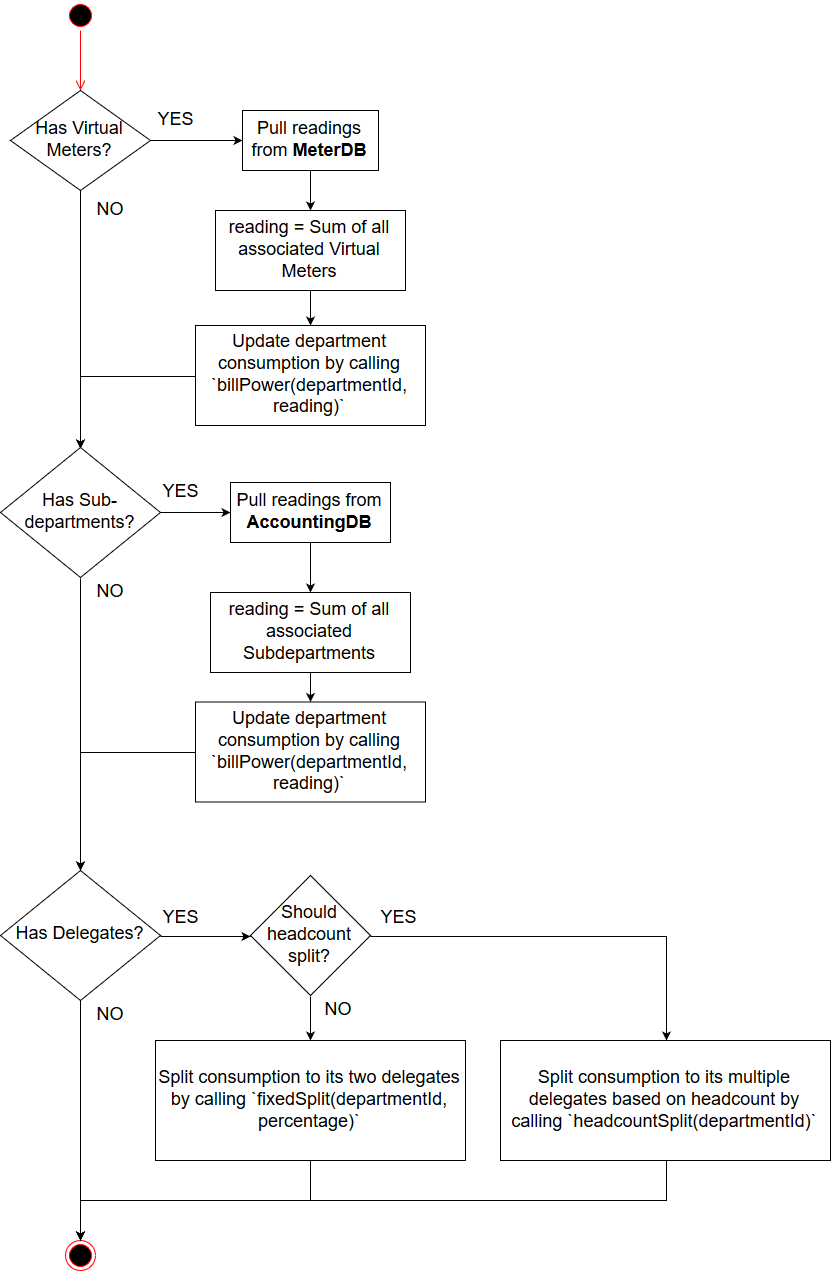
\includegraphics[width=\textwidth]{flowchart}
    \caption{Consumption calculation for a Department}
    \label{fig:consumption_flowchart}
\end{figure}

\subsection{Execution Pipeline} \label{execution}

Having described how each module of the client side works, in \ref{fig:execution} we show the order in which the client side programs get executed to provide the desired metering and billing functionality. Firstly, the administrator grants all of the needed privileges to the corresponding operators' addresses. The meter operator activates all meters, and all virtual meers. The accounting operator activates and initializes the accounting settings for each department. Each meter and virtual meter starts pushing their values asynchronously to the \texttt{MeterDB} contract, while at the same time the accountant is able to bill each department according to the logic which was previously specified by the accounting operator.

\begin{figure}[htb]
    \centering
    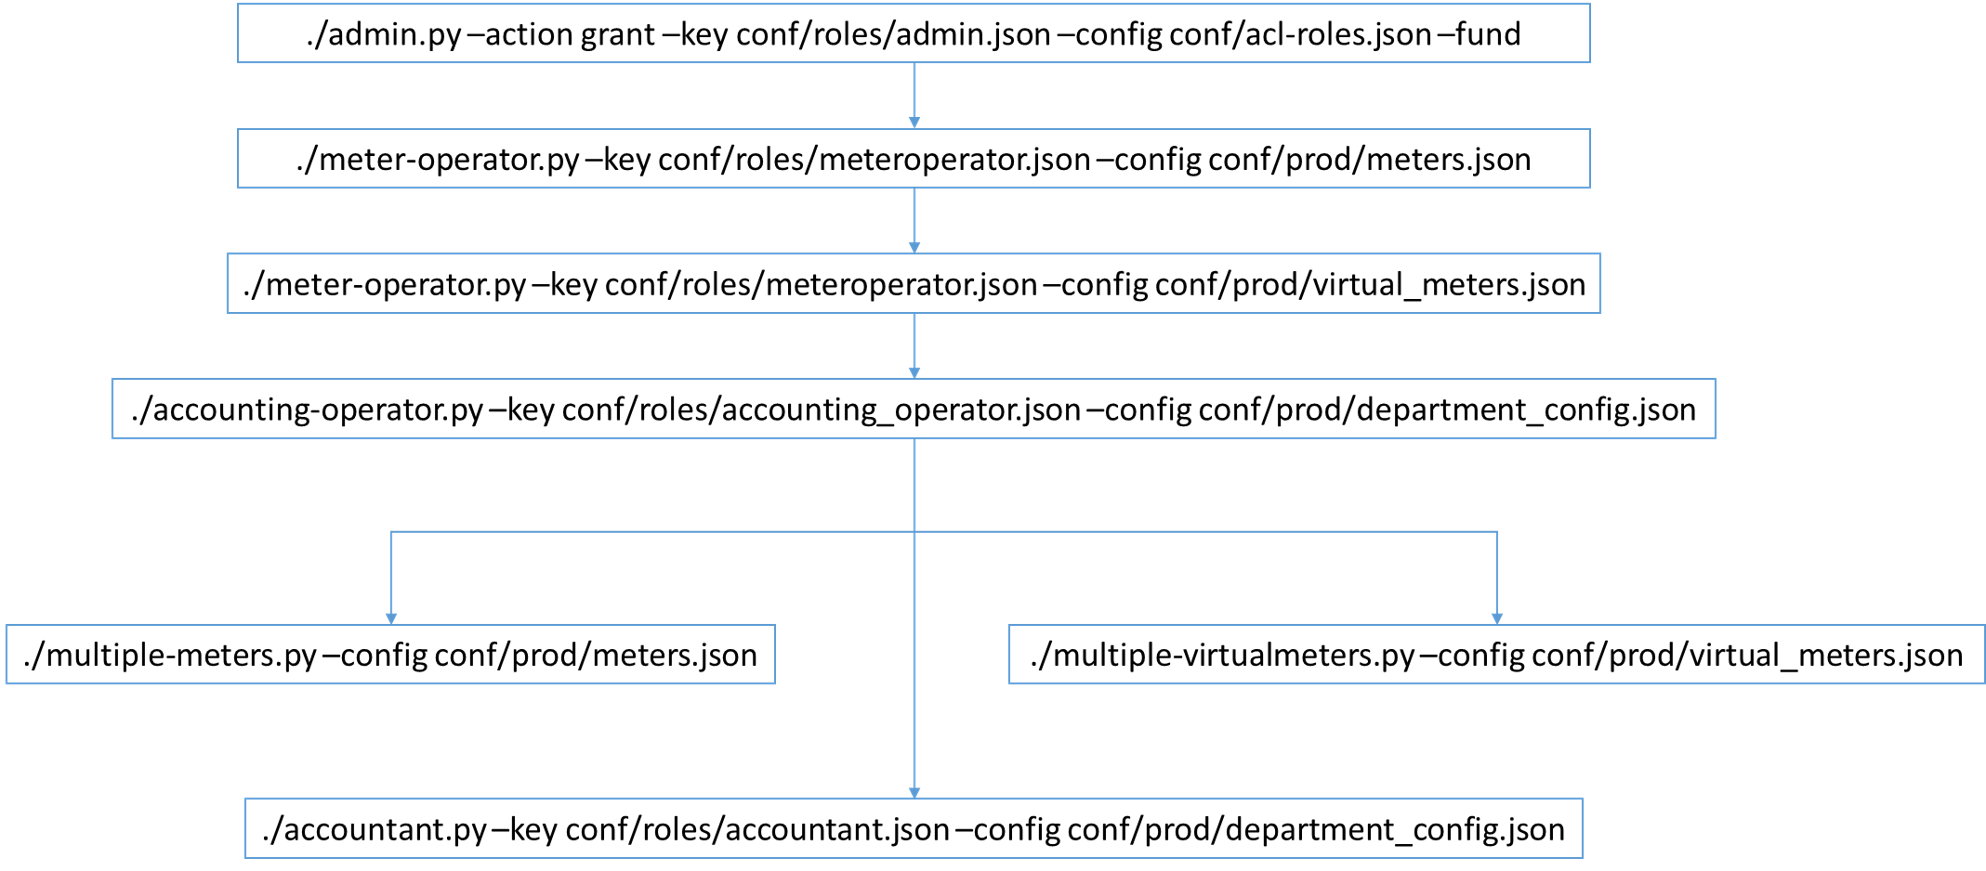
\includegraphics[width=\textwidth]{execution}
    \caption{The full execution process of metering and billing}
    \label{fig:execution}
\end{figure}

\chapter{Evaluation of Implementation and Results}\label{ch:results}

We have described an ecosystem of smart contracts that combined with their corresponding client scripts can perform metering and billing of energy on complex business logic. The energy billing per department is done in kilowatthours because there was no specified method of calculating the cost in fiat currency. Converting the measured energy to a fiat currency during the billing process is done outside of the proposed system, without loss of generality. We proceed to evaluate the performance of the implementation of Chapter \ref{ch:implementation}, and explain how the findings from Chapter \ref{ch:scalability} and Chapter \ref{ch:security} are applied to enable better scalability and robustness in the contract design.

\section{Scalability}
On scalability, we applied Method 3 (\ref{method3}) and followed the rules from Section \ref{gas-costs} to save gas. More specifically:

\begin{enumerate}
    \item The optimizer was run 200 times, which was the default option for the Truffle Framework.
    \item Using libraries via Method 3 for storing meter readings and department values resulted in significant code reuse, and reduction of gas costs. Table \ref{table:compare-gas} illustrates the gas savings that the proposed method provides, for each function of the contracts\footnote{The ACL logic was removed for these calculations.}.
    \item Any meter, department that is no longer used can be deactivated, freeing up storage in the smart contract.
    \item Any iterations over arrays are initializing the break condition outside of the loop, reducing the number of \texttt{SLOAD} operations done and thus saving gas.
    \item In all cases, \texttt{string} is avoided and \texttt{bytes32} is used. If a representation was needed that was larger than 32 bytes would be needed, it would be rendered in the front end by matching the 32 bytes to a potential string. 
    \item The minimal amount of data needed is stored in the smart contract. The latest reading and timestamp values are needed for each meter and department, and each department additionally requires storing its hierarchical relationship with other departments, virtual meters and its delegates. The formula for each virtual meter (\ref{metering}) is stored locally because it would significantly increase gas costs to store an arbitrarily long \texttt{string} variable in the smart contract.
    \item Events are emitted for each action providing an inexpensive way to store the historical data of a meter or department. Emitting an event requires 2000 gas, compared to the 20000 gas needed for storing a value. The disadvantage is that event data cannot be accessed by another smart contract which is acceptable in this case as historical data is only meant to be accessed by a client and not a smart contract directly. 
\end{enumerate}

\begin{table}[htb]
	\centering
	\caption{Gas costs comparison between Method 1 and Method 3 for storing meter readings and department energy consumptions, optimizer runs = 200}
	\vspace*{-1ex}
	\scriptsize
	\vspace{-1ex}
	\begin{tabular}{|c|c|c|c|}
		\hline
		\textbf{Contract} & \textbf{Method 1} & \textbf{Method 3} & \textbf{Improvement} \\ \hline
		MeterDB::deployment		      &    793279 &   637403 & 20\% \\
		AccountingDB::deployment      &    1691164 &   1088253   & 36\%\\
		MeterDB::ping 			      &    57844 &   31422   & 46\% \\
        AccountingDB::billPower       &    82025 &   28250   & 65\%\\
        AccountingDB::fixedSplit      &    98126 &   47260   & 51\%\\
        AccountingDB::headcountSplit  &    231305 &   55024   & 76\%\\
		\hline
	\end{tabular}
	\vspace{-2ex}
	\label{table:compare-gas}
\end{table}

\section{Security}

Having studied and understood past literature as well as attacks on smart contracts, the implementation is developed so that none of the known attacks can be reproduced. In Section \ref{slither} we evaluated that Slither can detect a wide variety of vulnerabilities, and can outperform at most cases the other available security auditing tools. Auditing our smart contracts through Slither showed no true positives, which given the past performance of the tool, gives us a high degree of confidence with regard to the robustness of the developed smart contracts against known attacks.

We utilized and applied an access control list to the implemented smart contracts which is able to enforce role based access control. Roles are given only access to specific functions of a smart contract that they must have access to, following the security principle of least privilege. Each user is then granted a role, which provides a modular method to revoke and modify the rules, in case of changes in the structure of an organization. Providing a way to enforce access control is important because smart contract ecosystems will become more complex as the requirements increase. More actors will need to be involved, and there will be a need to limit the functionality of each actor. In addition, it is not efficient to modify the permissions of each actor on a per-contract basis, and as a result a central directory of permissions needs to exist. In the past, as described in Section \ref{past-attacks}, lack of proper access control cost large amounts of funds to the involved parties.

\section{Complete overview}
The final implementation was tested with a setup of 48 smart meters, 44 virtual meters and 20 departments. The simulation was conducted on a Dell Laptop and consumed less than 10\% of the laptop's CPU and RAM resources, which illustrates how lightweight it is. The deployment of the smart contracts was firstly tested on a local ganache testnet instance, then on a locally deployed testnet of 2 geth instances, where 1 was acting as a node and another as a miner, and finally on the Ropsten public testnet. Due to company requirements, there was no deployment to a public network, however the contract design allows that. 

The operating costs are correlated linearly to the frequency that the data is pushed to the smart contracts. 

\begin{enumerate}
    \item \textbf{Meters:} The monitoring server is updated every 12 minutes, however since the change in values is very small, we poll the monitoring server and update the values of the smart meters every 2 hours\footnote{The selected frequency was a company requirement. Further granularity provided no advantage. It is possible to push values every 12 minutes, at a linear increase in cost}. As a result, the operating cost for pinging the values of 48 meters for a year\footnote{The chosen gas price is $1 GWei = 10^{-9} ether$ since the operations are not time critical. When there is a need for fast confirmations the price is expected to be higher.} is: 48 meters * 31422 gas * 0.5 readings / hour * 24 hours * 365 days * 1 Gwei/gas  = 6.6 ether, which reduces to each meter needing 0.1375 ether in order to be able to interact with the smart contract at the specified frequency for a year. 
    \item \textbf{Virtual Meters:} Pushing the values of Virtual Meters is required to be done twice every month and so the total cost of running 44 virtual meters is: 44 virtual meters * 31422 gas * 2 readings / month * 12 months * 1 Gwei/gas  = 0.03 ether, which reduces to each virtual meter needing 0.0007 ether to interact with the smart contract at the specified frequency for a year. 
    \item \textbf{Billing:} Calculating the consumption of each business unit and performing cost forwarding for internal accounting is required to be done once every month. It was simulated that a full billing cycle of pulling values from virtual meters, updating each department's consumption and delegating it according to the business logic costs X ether per month, or X ether per year. 
\end{enumerate}

\chapter{Conclusion}\label{ch:conclusion}

\section{Future Work}
The main issue with our curernt implementation is that instead of having a direct push from each meter (or any IoT device) to the blockchain, we need to pull the data from the aforementioned monitoring server, and then push it again. This introduces latencies and single points of failure, however, this was done due to our corporate setup. An improvement would be to setup a microcontroller on each that would be executing a binary that pings readings to the blockchain. even better, run a node on each IOt device, however requires too much power, maybe in the far future. We explore Ethereum platform due to its abundance in developers and stay in it. There are other smart contract platforms however they lack developer tools, are not battle tested and are potentially centralized. As there is a bigger issue with scaling, the whole infrastructure could be transferred to a permissioned in-house blockchain, however we wanted to stay within the scope of keeping it as transparent as possible.

FIN.



\bibliographystyle{ieeetr}
\bibliography{references}

% \printglossaries
\listoffigures
\listoftables

\begin{appendices}

\chapter{Transactions and Blocks}
Querying a node for transactions:
\begin{figure}[H]
    \centering
    \lstinputlisting{code/transaction_example.json}
    \caption{Contents of an Ethereum transaction when querying a node}
    \label{fig:transaction}
\end{figure}

Querying a node for block contents:
\begin{figure}[H]
    \centering
    \lstinputlisting{code/block_example.json}
    \caption{Contents of an Ethereum block when querying a node}
    \label{fig:block}
\end{figure}

Ganache UI:
\begin{figure}[H]
    \centering
    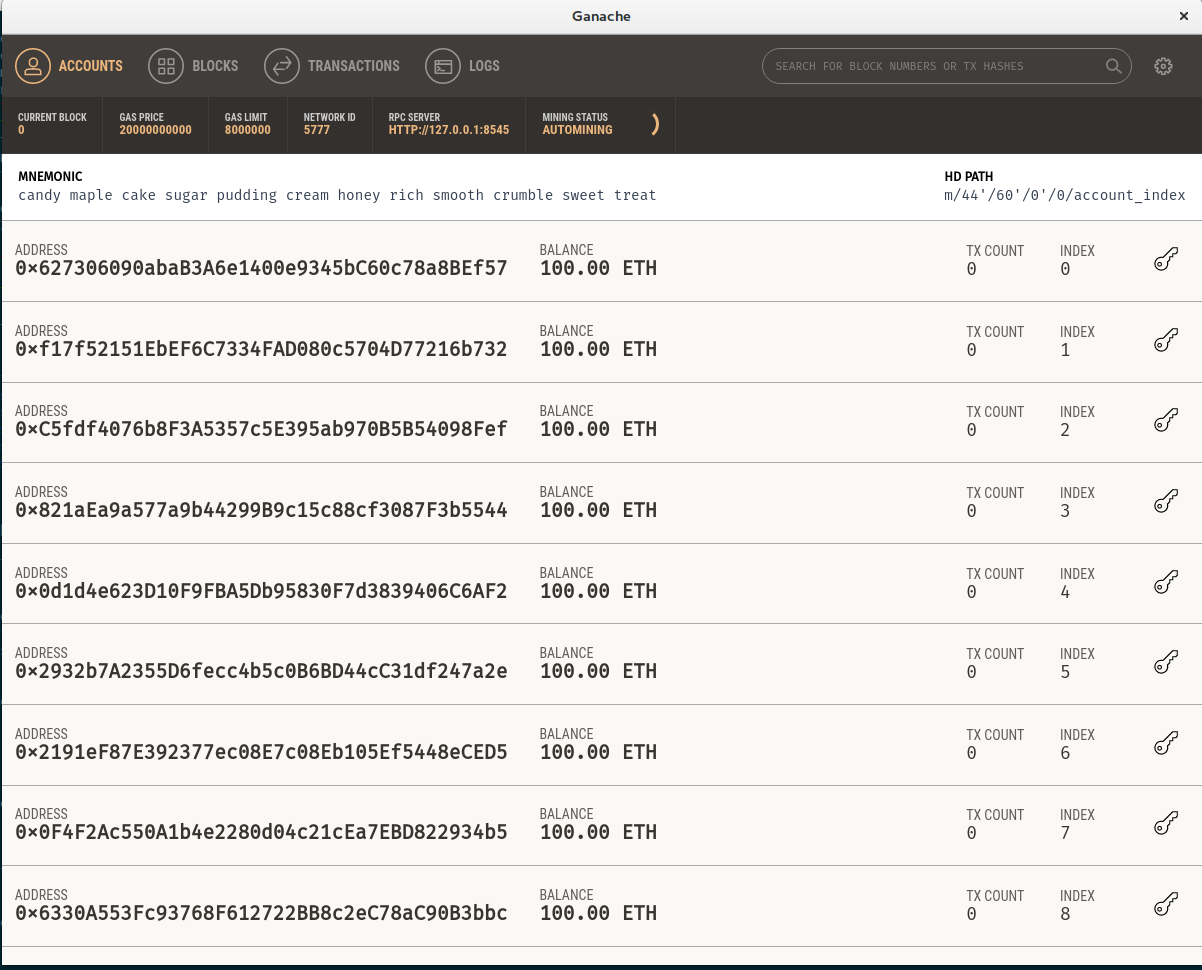
\includegraphics[width=1.0\textwidth]{ganache}
    \caption{Ganache testnet User Interface}
    \label{fig:ganache}
    
\end{figure}

Web3js example:
\begin{figure}[H]
    \centering
    \lstinputlisting{code/web3.js}
    \caption{Interacting with a node in Javascript}
    \label{fig:web3js}
\end{figure}

Web3py example:
\begin{figure}[H]
    \centering
    \lstinputlisting{code/web3.py}
    \caption{Interacting with a node in Python}
    \label{fig:web3py}
\end{figure}

\chapter{Scalability through Gas Saving masks} \label{apx:scalability}

\begin{figure}[ht!]
    \centering
    \lstinputlisting[language=Solidity]{contracts/LibraryExample.sol}
    \caption{Example of using the \texttt{using X for Y} syntax to enhance operations done on datatypes.}
    \label{fig:library}
\end{figure}


\begin{figure}[ht!]
    \centering
    \lstinputlisting[language=Solidity]{contracts/LibraryExample.sol}
    \caption{Example of using the \texttt{using X for Y} syntax to enhance operations done on datatypes.}
    \label{apx:scalability:overflow}
\end{figure}



\begin{figure}[H]
  \begin{subfigure}[b]{\textwidth}
    \centering
    \lstinputlisting[language=Solidity]{contracts/Packing.sol}
  \end{subfigure}

  \begin{subfigure}[b]{\textwidth}
    \centering
    \lstinputlisting{code/solc.txt}
  \end{subfigure}
  \caption{Running the optimizer in storage variables less than 256 bytes results in 2 SSTORE commands instead of 6 which reults in significant savings in gas costs}
  \label{fig:struct_optimization}
\end{figure}
Game interface:
\begin{figure}[H]
    \centering
    \lstinputlisting[language=Solidity]{contracts/GameInterface.sol}
    \caption{Interface for described use-case}
    \label{fig:game_interface}
\end{figure}

Tightly packed code:
\begin{figure}[H]
  % Struct Definition
  \begin{subfigure}[b]{\textwidth}
    \centering
    \lstinputlisting[language=Solidity, firstline=4, lastline=13]{contracts/GameTightlyPacked.sol}
    \caption{Character structure definition}
    \label{fig:struct_optimization:a}
  \end{subfigure}

  \begin{subfigure}[b]{\textwidth}
    \centering
    \lstinputlisting[language=Solidity, firstline=38, lastline=66]{contracts/GameTightlyPacked.sol}
    \caption{Create character simply sets values to each struct variable}
    \label{fig:struct_optimization:b}
  \end{subfigure}
\end{figure}

\begin{figure}[H] \ContinuedFloat
  \begin{subfigure}[b]{\textwidth}
    \centering
    \lstinputlisting[language=Solidity, firstline=68, lastline=92]{contracts/GameTightlyPacked.sol}
    \caption{Retrieve the character and save it in memory, then return all values.}
    \label{fig:struct_optimization:c}
  \end{subfigure}
  \caption{Implementation requires a Solidity `struct' to pack all the variables together. CreateCharacter and GetCharacterStats  }
  \label{fig:struct_optimization}
\end{figure}

Method 2 code:

\begin{figure}[H]
    \centering
    \lstinputlisting[language=Solidity, firstline=10, lastline=36]{contracts/GameByteMasking.sol}
    \caption{Create Character by shifting variables}
    \label{fig:uint_encoding_code}
\end{figure}

\begin{figure}[H] 
    \centering
    \lstinputlisting[language=Solidity, firstline=38, lastline=61]{contracts/GameByteMasking.sol}
    \caption{Get the traits of a character by shifting and masking appropriately. Typecasting is the same as applying a mask of $N$ bits.}
    \label{fig:uint_decoding_code}
\end{figure}

Method 3 code:

\begin{figure}[H]
  \begin{subfigure}[b]{\textwidth}
    \centering
    \lstinputlisting[firstline=35, lastline=41, language=Solidity]{contracts/GameByteMaskingLib.sol}
    \caption{Getting and setting a property}
  \end{subfigure}
  \begin{subfigure}[b]{\textwidth}
    \centering
    \lstinputlisting[linerange={21-21,26-26}, language=Solidity]{contracts/GameByteMaskingLib.sol}
    \caption{Mask and shift offsets for CreationTime}
  \end{subfigure}
  \begin{subfigure}[b]{\textwidth}
    \centering
    \lstinputlisting[linerange={44-44,53-53}, language=Solidity]{contracts/GameByteMaskingLib.sol}
    \caption{Getting and Setting creation time API}
  \end{subfigure}
  \caption{Parts of the Library API for Character Creation}
  \label{apx:scalability:lib}
\end{figure}

\begin{figure}[H]
    \begin{subfigure}[b]{0.5\textwidth}
        \centering
        \lstinputlisting[language=Solidity, linerange={101-108}]{contracts/GameByteMaskingLib.sol}
        \caption{Create Character by shifting variables}
        \label{fig:bytes_encoding_code}
    \end{subfigure}
    \begin{subfigure}[b]{0.5\textwidth}
        \centering
        \lstinputlisting[language=Solidity, linerange={129-139}]{contracts/GameByteMaskingLib.sol}
        \caption{get character variables}
        \label{fig:bytes_decoding_code}
    \end{subfigure}
\end{figure}

\chapter{Security}
\begin{figure}[H]
    \centering
    \lstinputlisting[language=Python]{code/getstorageat.py}
    \caption{Inspecting the first storage slot of a contract}
    \label{fig:storage}
\end{figure}
\chapter{Code for Smart Meters}

\end{appendices}


\end{document}